% =========================================================
%  Chapter 4 -- The Laser Oscillator
%  Style: student-voice notes matching the personal style guide
% =========================================================

At the end of the previous chapter, we confronted the fundamental limitation of the travelling-wave amplifier: despite containing massive amounts of stored atomic energy via population inversion, it is ultimately just a powerful optical megaphone waiting for a voice. It strictly requires an external seed signal to trigger stimulated emission.

In this chapter, we eliminate the need for an external input entirely. By taking that exact same active gain medium and trapping it inside a resonant optical cavity---between two highly reflective mirrors---we introduce \textbf{optical feedback}. A few initially random, spontaneously emitted photons will now become trapped and bounce back and forth, triggering a massive avalanche of stimulated emission on every pass. By closing the loop, we have transformed our open-loop amplifier into a self-sustained \textbf{laser oscillator} (Light Amplification by Stimulated Emission of Radiation).

\begin{figure}[H]
    \centering
    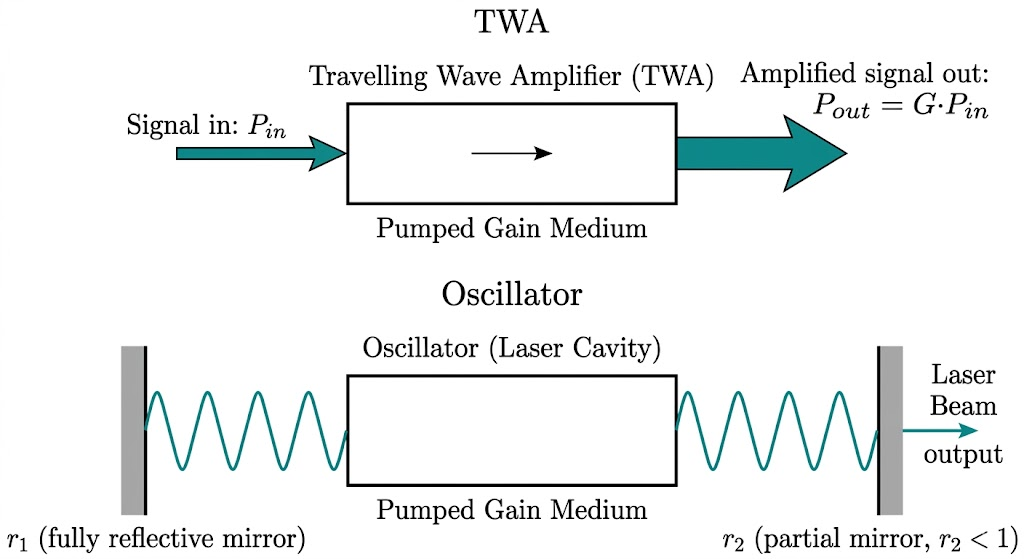
\includegraphics[width=0.6\textwidth]{Figures/Chapter 4/twa_vs_oscillator.jpg}
    \caption{From Amplifier to Oscillator: A single-pass Travelling-Wave Amplifier requires an external seed signal and provides no feedback. Adding two mirrors to form a Fabry-P\'{e}rot cavity traps the light inside the gain medium, enabling self-sustained oscillation without any external input.}
\end{figure}

Our primary goal in this chapter is to understand the exact mechanics of this transformation. We must map how trapping an active gain medium inside a geometrical cavity dictates the fundamental oscillation conditions, the allowed mode frequencies, the threshold pump rate, and the final output power of a running laser.

% ----------------------------------------------------------
%  Section 1: The Mechanics of the Laser Oscillator
% ----------------------------------------------------------
\section{The Mechanics of the Laser Oscillator}

\subsection{The Three Conditions for Oscillation}

A laser is, at its core, an oscillator in the strict engineering sense. Just like any electronic or mechanical oscillator, it requires exactly three functional components to successfully generate a stable, self-sustaining signal. In a laser, each of these abstract requirements maps directly to a physical optical mechanism we have already derived:

\begin{enumerate}
    \item \textbf{A Noise Source (Spontaneous Emission):} Every oscillator needs an initial seed to spark the process. In a laser, this seed is provided by random spontaneous emission from the excited atoms. While these photons are initially fired in random directions and phases, the tiny fraction that happen to emit directly along the longitudinal cavity axis get amplified and eventually dominate the entire intracavity field.

    \item \textbf{A Selective Feedback Mechanism (The Fabry-P\'{e}rot Cavity):} Feedback routes the optical output directly back to the input. We achieve this by placing two mirrors facing each other across the gain medium, forcing photons to bounce back and forth and accumulate exponential gain on every pass. This mirror assembly (the Fabry-P\'{e}rot resonator) also acts as an aggressive frequency filter: only the discrete resonant modes of the cavity experience constructive round-trip interference and survive.

    \item \textbf{A Stabilising Nonlinearity (Gain Saturation):} If the round-trip gain stayed mathematically above unity forever, the intracavity power would grow toward infinity. To prevent this, the system relies on the saturation physics we derived previously:
          \begin{equation*}
              \gamma = \frac{\gamma_0}{1 + \Phi/\Phi_s}
          \end{equation*}
          As the photon flux $\Phi$ builds up inside the cavity, it rapidly depletes the population inversion, forcing the overall gain coefficient $\gamma$ downward. The oscillation ultimately stabilises at a finite, perfectly balanced steady-state power where the saturated intracavity gain exactly equals the physical cavity losses.
\end{enumerate}

% ----------------------------------------------------------
%  The Fabry-Perot Cavity -- Round-Trip Analysis
% ----------------------------------------------------------
\subsection{The Fabry-P\'{e}rot Cavity --- Round-Trip Analysis}

Now let's talk about the heart of the laser: the Fabry-P\'{e}rot resonator. The cavity consists of a gain medium of length $L$ between two mirrors $M_1$ and $M_2$ with field reflectivities $r_1$ and $r_2$ (and power reflectivities $R_1 = r_1^2$ and $R_2 = r_2^2$). The gain medium has gain coefficient $\gamma$ and internal loss coefficient $\alpha_s$ (which accounts for scattering and non-resonant absorption, since resonant absorption by the lasing atoms is inherently handled by the net gain coefficient $\gamma$).

We start by asking what happens to the electric field amplitude as it completes one full round trip. Let the field amplitude at a reference point just inside mirror $M_1$ be $E_1$. We follow it step by step.

The field propagates from $M_1$ to $M_2$ over length $L$, accumulating a phase factor $e^{-j\beta L}$ and an amplitude factor $e^{-\alpha_s L/2}\,e^{\gamma L/2}$ (one-half exponents convert from power to field amplitude):
\begin{equation*}
    E_2 = E_1\,e^{-j\beta L}\,e^{(\gamma - \alpha_s)L/2}
\end{equation*}

The field then reflects off $M_2$ with field reflectivity $r_2$:
\begin{equation*}
    E_3 = r_2\,E_1\,e^{-j\beta L}\,e^{(\gamma - \alpha_s)L/2}
\end{equation*}

It propagates back from $M_2$ to $M_1$, picking up the same exponential factors again:
\begin{equation*}
    E_4 = r_2\,E_1\,e^{-j2\beta L}\,e^{(\gamma - \alpha_s)L}
\end{equation*}

Finally, it reflects off $M_1$ with field reflectivity $r_1$:
\begin{equation*}
    E_5 = r_1 r_2\,E_1\,e^{-j2\beta L}\,e^{(\gamma - \alpha_s)L}
\end{equation*}

After one complete round trip, the returned field $E_5$ is related to the starting field $E_1$ by the round-trip multiplication factor:
\begin{equation*}
    \frac{E_5}{E_1} = r_1 r_2\,e^{-j2\beta L}\,e^{(\gamma - \alpha_s)L}
\end{equation*}

For sustained oscillation we need $E_5 = E_1$ --- the field must reproduce itself exactly after every round trip. This single vector equation splits into a phase condition and an amplitude condition, which we now derive separately.

\begin{figure}[H]
    \centering
    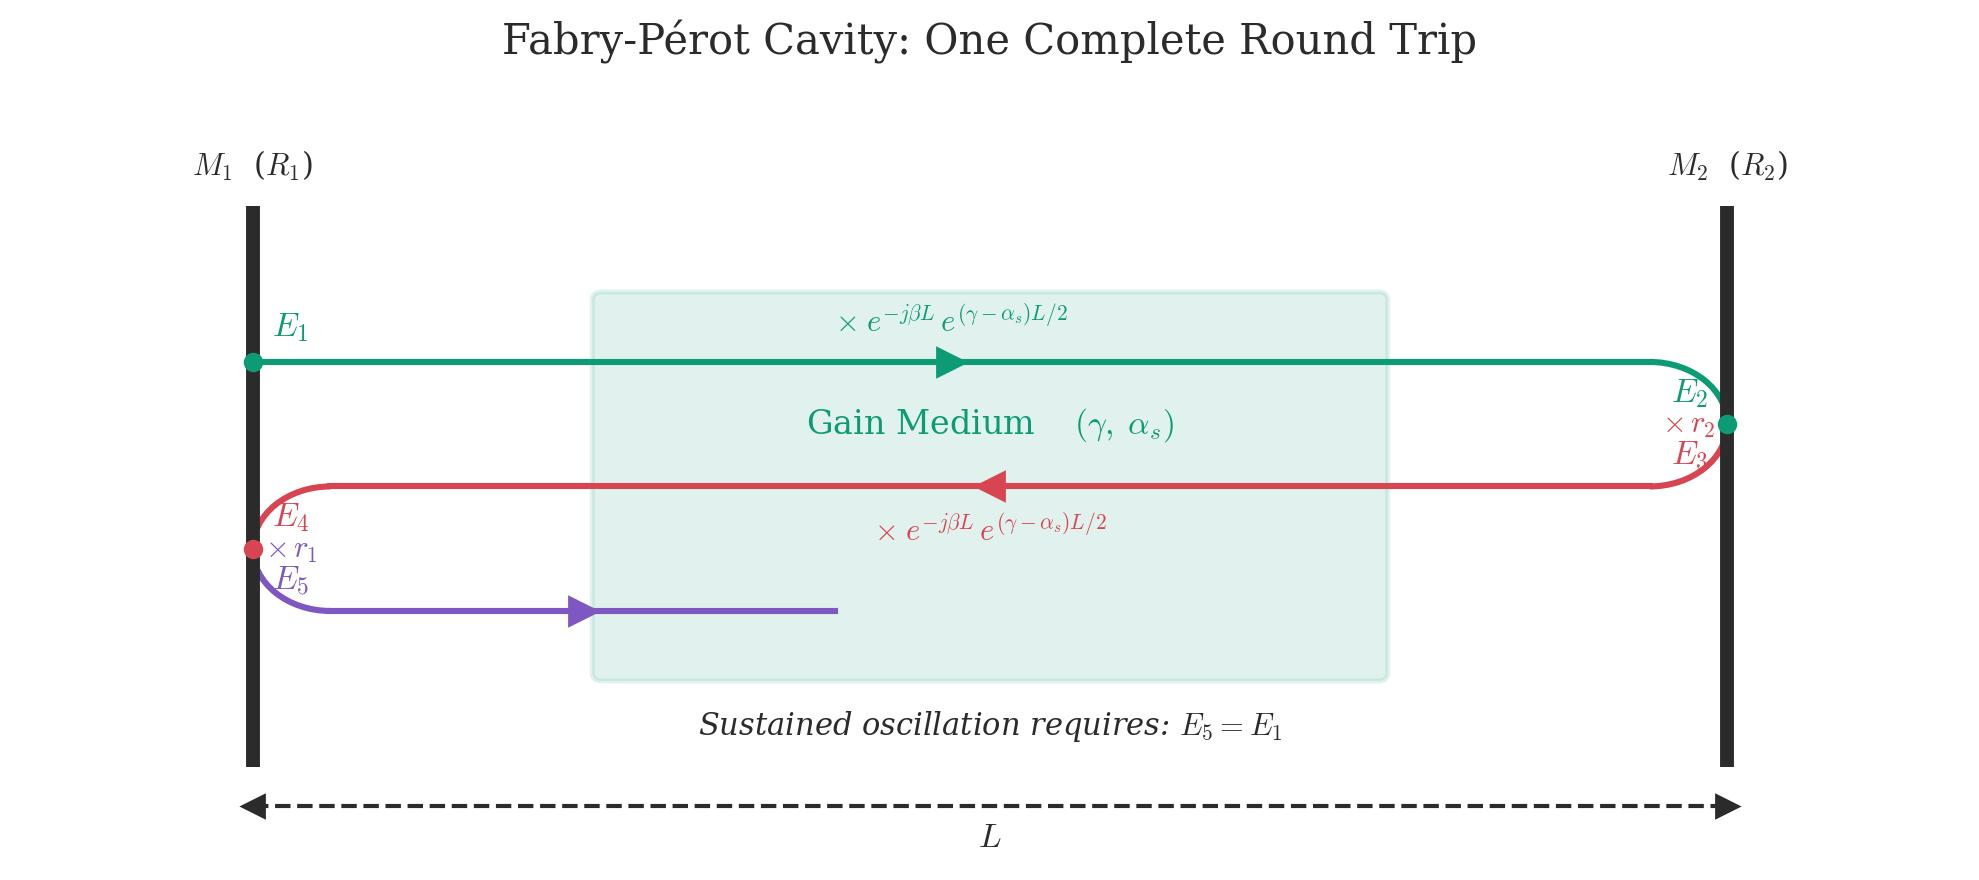
\includegraphics[width=0.6\textwidth]{Figures/Chapter 4/fp_cavity_round_trip.jpg}
    \caption{Fabry-P\'{e}rot Cavity Round Trip: The electric field amplitude at each stage of one complete round trip, from $E_1$ (reference) through forward propagation $E_2$, reflection $E_3$, backward propagation $E_4$, and final reflection $E_5$. Sustained oscillation requires the field amplitude and phase to reproduce exactly: $E_5 = E_1$.}
\end{figure}

\subsubsection{The phase condition --- longitudinal modes}

For $E_5 = E_1$, the complex round-trip factor must equal exactly one. The phase part of this requirement is:
\begin{equation*}
    e^{-j2\beta L} = 1
\end{equation*}

This holds only when the round-trip phase is an integer multiple of $2\pi$:
\begin{equation*}
    2\beta L = 2q\pi, \qquad q = 1,\,2,\,3,\,\ldots
\end{equation*}

The propagation constant in a medium is $\beta = 2\pi\nu/c$. Substituting this (and using $\nu_q$ instead of $\nu$ to denote the discrete allowed frequencies):
\begin{equation*}
    2\cdot\frac{2\pi\nu_q}{c}\cdot L = 2q\pi
\end{equation*}
Solving for $\nu_q$:
\begin{keyresult}
    \begin{equation}
        \nu_q = q\cdot\frac{c}{2L}, \qquad q = 1,\,2,\,3,\,\ldots
    \end{equation}
\end{keyresult}
where:
\begin{itemize}
    \item $\nu_q$: the frequency of the $q$-th \textbf{longitudinal mode} of the cavity.
    \item $q$: the longitudinal mode number (an integer; in practice $q \sim 10^5$--$10^6$ for optical cavities).
    \item $c$: the speed of light in the medium.
\end{itemize}

Only these discrete frequencies satisfy the phase condition. At any other frequency, successive round trips interfere destructively and the field dies. These $\nu_q$ are called the \textbf{cold-resonator modes} because they depend only on the cavity geometry --- not on the gain medium. The phase condition is purely a geometric constraint: the round-trip path length $2L$ must contain exactly $q$ whole wavelengths in the medium.

\subsubsection{The amplitude condition --- threshold gain $\alpha_r$}

To sustain or build up oscillation, the field amplitude must not decay after a round trip. Therefore, the amplitude part of the round-trip condition requires $|E_5| \geq |E_1|$, which means:
\begin{equation*}
    \left|r_1 r_2\right|\cdot e^{(\gamma - \alpha_s)L} \geq 1
\end{equation*}

Taking the natural logarithm of both sides:
\begin{equation*}
    \ln(r_1 r_2) + (\gamma - \alpha_s)L \geq 0
\end{equation*}

Since $r_i = \sqrt{R_i}$, we have $\ln(r_1 r_2) = \tfrac{1}{2}\ln(R_1 R_2)$. Rearranging for $\gamma$:
\begin{equation*}
    \gamma L \geq \alpha_s L - \tfrac{1}{2}\ln(R_1 R_2) \quad\implies\quad \gamma L \geq \alpha_s L + \tfrac{1}{2}\ln\!\left(\frac{1}{R_1 R_2}\right)
\end{equation*}

Dividing through by $L$, we find the condition that the gain must satisfy to sustain oscillation:
\begin{equation*}
    \gamma \geq \alpha_s + \frac{1}{2L}\ln\!\left(\frac{1}{R_1 R_2}\right)
\end{equation*}

The right-hand side is a fixed geometric constant. We define this exact boundary value as the \textbf{threshold gain} ($\gamma_{\text{th}}$), which is equal to the \textbf{total loss coefficient} ($\alpha_r$):
\begin{keyresult}
    \begin{equation}
        \gamma_{\text{th}} = \alpha_s + \frac{1}{2L}\ln\!\left(\frac{1}{R_1 R_2}\right) \equiv \alpha_r
    \end{equation}
\end{keyresult}
where:
\begin{itemize}
    \item $\alpha_r$: the \textbf{total loss coefficient} --- the gain per unit length that must be achieved to sustain oscillation.
    \item $\alpha_s$: the internal scattering and \textit{non-resonant} absorption loss per unit length inside the cavity.
    \item $\frac{1}{2L}\ln(1/R_1 R_2)$: the effective distributed loss per unit length due to useful power leaking out through the mirrors --- the \textbf{output coupling loss}.
\end{itemize}

The amplitude condition states: the gain coefficient must meet or exceed $\alpha_r$ to sustain oscillation. If $\gamma < \alpha_r$, the field decays after each round trip; if $\gamma > \alpha_r$, the field grows.

This sets up a strict, self-regulating feedback loop known as \textbf{gain clamping}. When the laser is first turned on, the pump raises the small-signal gain well above the loss ($\gamma_0 > \alpha_r$). Because gain exceeds loss, the intracavity photon flux grows exponentially. However, as the photon population explodes, it stimulates emission at a massive rate, rapidly eating away the excited atoms. This depletion of the population inversion physically forces the operating gain $\gamma$ to drop (a process called gain saturation).

The field continues to grow---and the gain continues to drop---until the gain falls to exactly match the cavity loss ($\gamma = \alpha_r$). At this precise moment, round-trip amplification perfectly balances round-trip loss, and the photon flux stops growing. The system locks into a steady state. If the gain were slightly higher, extra photons would be generated, which would instantly deplete the gain back down. If the gain dropped slightly lower, photons would die out, allowing the continuous pumping to rebuild the gain back up. Therefore, the steady-state operating gain is strictly clamped to $\alpha_r$.

\subsubsection{Photon lifetime}

To complete our characterisation of the cavity, we can derive the \textbf{photon lifetime} $\tau_{\text{ph}}$ --- the average time a photon survives inside the cavity before being lost through the mirrors or internal scattering. Inside the lossy passive cavity, the optical intensity decays spatially under the combined distributed loss $\alpha_r$:
\begin{equation*}
    I(z) = I(0)\,e^{-\alpha_r z}
\end{equation*}

To translate this spatial decay into a temporal one, we apply the chain rule. The disturbance travels at the group velocity $v_g$ of the optical mode, so $dz/dt = v_g$:
\begin{equation*}
    \frac{dI}{dt} = \frac{dI}{dz}\cdot\frac{dz}{dt} = (-\alpha_r I)\cdot v_g = -\alpha_r v_g\,I
\end{equation*}

Integrating this separable ODE:
\begin{equation*}
    I(t) = I(0)\,e^{-\alpha_r v_g\,t}
\end{equation*}

Reading off the exponential time constant:
\begin{keyresult}
    \begin{equation}
        \tau_{\text{ph}} = \frac{1}{\alpha_r\,v_g}
    \end{equation}
\end{keyresult}

The mode linewidth is directly tied to the photon lifetime by the time-frequency uncertainty of a decaying exponential:
\begin{keyresult}
    \begin{equation}
        \delta\nu = \frac{1}{2\pi\,\tau_{\text{ph}}}
    \end{equation}
\end{keyresult}

The mode linewidth is thus $\delta\nu = 1/(2\pi\tau_{\text{ph}}) = \alpha_r c/(2\pi)$. A tightly confining, low-loss cavity enjoys a long photon lifetime and sharply defined narrow modes; a lossy cavity suffers a short photon lifetime and bleeds into broad modes.

The physical significance of the photon lifetime goes far beyond a passive decay constant; it directly dictates the \textbf{ON/OFF switching dynamics} and maximum modulation speed of the laser oscillator:
\begin{itemize}
    \item \textbf{Turn-Off Speed (Decay):} When the pump current is abruptly switched off, the intracavity field cannot vanish instantaneously. The trapped photons continue to escape the mirrors, and the light intensity decays exponentially as $I(t) = I(0)\,e^{-t/\tau_{\text{ph}}}$. A long photon lifetime (desirable for high-confinement, low-threshold cavities) therefore acts as a temporal bottleneck, slowing down the decay speed.
    \item \textbf{Turn-On Delay (Build-up):} Similarly, when the pump is suddenly turned on, the laser does not emit light instantly. It requires a finite build-up delay for spontaneous emission photons to bounce back and forth, accumulating enough round-trip gain to surpass losses and establish the steady-state flux. This build-up time is fundamentally scaled by $\tau_{\text{ph}}$.
    \item \textbf{The Modulation Trade-off:} Consequently, for high-speed digital communications where the laser must switch between logical 1 and 0 at gigahertz rates, designers must intentionally decrease $\tau_{\text{ph}}$ (by reducing mirror reflectivities $R_i$), even though this undesirable change increases the required threshold pump rate $R_{\text{th}}$.
\end{itemize}

The phase and amplitude conditions, along with the photon lifetime, completely characterise the mechanics of the laser oscillator. We now look at the physical hardware used to trap this light.


% ----------------------------------------------------------
\subsection{Types of Mirrors}

Since the mirrors appear explicitly in the threshold gain condition through $R_1 R_2$, it is worth pausing to understand what kinds of mirrors are used in practice.

\subsubsection{Simple discontinuity}

The simplest mirror is an abrupt interface between two media with different refractive indices. At a planar boundary between media with indices $n_1$ and $n_2$, the Fresnel formula gives the field reflectivity at normal incidence:
\begin{equation*}
    r = \frac{n_2 - n_1}{n_2 + n_1}
\end{equation*}

For a semiconductor-air interface with $n_2 = n$ (semiconductor) and $n_1 = 1$ (air):
\begin{equation*}
    r = \frac{n - 1}{n + 1}, \qquad R = \left(\frac{n-1}{n+1}\right)^{\!2}
\end{equation*}

For a typical semiconductor with $n \approx 3.5$, this gives $R \approx 31\%$, which is often sufficient to sustain laser oscillation without any additional coating. This is how the simplest semiconductor laser diodes are constructed --- the cleaved facets of the semiconductor chip act as the two mirrors.

\subsubsection{Free-standing dielectric mirror}

A more versatile option is a free-standing dielectric mirror --- a thin slab or multilayer stack of dielectric material placed in the cavity. By choosing the thicknesses and refractive indices appropriately, almost any desired reflectivity $R(\lambda)$ can be engineered over a chosen wavelength range. This gives the laser designer fine control over both the output coupling loss and the frequency selectivity of the cavity.

With the mirror types established, the cavity geometry and mirror loss are fully specified. We can now return to the threshold condition and ask how much population inversion --- and therefore how much pumping --- is required to raise the gain to $\alpha_r$.

% ----------------------------------------------------------
%  Section 2: Threshold Pumping, Mode Selection, and Output Power
% ----------------------------------------------------------
\section{Threshold Pumping, Mode Selection, and Output Power}

\subsection{Threshold Population Inversion}

We now know what $\alpha_r$ is and what the gain must equal for oscillation to begin. The next question is: how large must the population inversion be --- and how hard must we pump --- to achieve $\gamma \geq \alpha_r$? We answer this by connecting the threshold gain to the threshold population inversion and then to the threshold pump rate.

The gain coefficient is related to the population inversion $N_0 = N_2 - N_1$ and the stimulated emission cross section $\sigma(\nu)$ by:
\begin{equation*}
    \gamma_0 = \sigma(\nu)\cdot N_0
\end{equation*}

At the lasing threshold, the small-signal gain must exactly equal the total cavity loss:
\begin{equation*}
    \gamma_{\text{th}} = \alpha_r \quad\Longrightarrow\quad \sigma(\nu)\,N_{0,\text{th}} = \alpha_r
\end{equation*}

Solving for the \textbf{threshold population inversion}:
\begin{keyresult}
    \begin{equation}
        N_{0,\text{th}} = \frac{\alpha_r}{\sigma(\nu)}
    \end{equation}
\end{keyresult}

This result is general. Strictly, $\sigma(\nu)$ should be evaluated at the first cavity mode that reaches threshold. In the usual dense-mode approximation, that mode lies very close to the atomic line centre $\nu_0$, where the gain is highest, so we use $\nu=\nu_0$ for a clean threshold estimate. The stimulated emission cross section at line centre for a Lorentzian lineshape of FWHM $\Delta\nu$ follows directly from the Einstein $B$-coefficient relation tied to the lineshape function $g(\nu_0) = 2/(\pi\Delta\nu)$:
\begin{equation*}
    \sigma(\nu_0) = \frac{\lambda^2}{8\pi\tau_{\text{sp}}}\cdot g(\nu_0)
    = \frac{\lambda^2}{8\pi\tau_{\text{sp}}}\cdot\frac{2}{\pi\,\Delta\nu}
    = \frac{\lambda^2}{4\pi^2\,\Delta\nu\,\tau_{\text{sp}}}
\end{equation*}

Substituting into the threshold inversion:
\begin{equation*}
    N_{0,\text{th}} = \alpha_r\cdot\frac{4\pi^2\,\Delta\nu\,\tau_{\text{sp}}}{\lambda^2}
\end{equation*}

Using the photon lifetime relation $\alpha_r = 1/(v_g\,\tau_{\text{ph}})$ with $v_g = c$ in the medium (derived above from the Fabry-P\'{e}rot linewidth):
\begin{keyresult}
    \begin{equation}
        N_{0,\text{th}} = \frac{4\pi^2\,\Delta\nu\,\tau_{\text{sp}}}{\lambda^2\,c\,\tau_{\text{ph}}}
    \end{equation}
\end{keyresult}

The physical message is transparent: a shorter photon lifetime (lossier cavity), a larger atomic linewidth, or a shorter in-medium wavelength all require a higher threshold inversion before lasing can begin.

\subsection{Threshold Pump Rate}

To find the threshold pump rate, we use the three-level laser rate equation results from the previous chapter. At steady state with no intracavity signal present, the small-signal population inversion established by the pump at rate $R$ is:
\begin{equation*}
    N_0 = 2R\,\tau_{21} - N_a
\end{equation*}
where $\tau_{21}$ is the spontaneous emission lifetime of the upper lasing level and $N_a$ is the total density of active atoms. Setting $N_0 = N_{0,\text{th}}$ and solving for the threshold pump rate:
\begin{equation*}
    2R_{\text{th}}\,\tau_{21} - N_a = N_{0,\text{th}} = \frac{\alpha_r}{\sigma(\nu_0)}
\end{equation*}
\begin{keyresult}
    \begin{equation}
        R_{\text{th}} = \frac{N_a}{2\tau_{21}} + \frac{\alpha_r}{2\sigma(\nu_0)\,\tau_{21}}
    \end{equation}
\end{keyresult}

The first term $N_a/(2\tau_{21})$ is the pump rate needed just to overcome the ground-state population and reach transparency ($N_2 = N_1$). The second term is the additional pumping required to push the inversion up to the level $N_{0,\text{th}}$ needed to overcome the cavity losses. Without any pumping, $\gamma$ is negative (absorption); as $R$ increases, $\gamma$ rises; at $R = R_{\text{th}}$, the gain at line centre just reaches $\alpha_r$ and laser oscillation begins. Further pumping above threshold builds up a large intracavity photon flux.

Once the pump has crossed threshold, the next question is no longer whether lasing is possible, but \emph{which} of the allowed longitudinal modes survive after gain saturation sets in.

% ----------------------------------------------------------
%  Mode Selection and Broadening in the Laser
% ----------------------------------------------------------
Now that we understand the conditions for lasing, we need to ask which frequencies actually lase. The phase condition allows only the discrete frequencies $\nu_q = q\,\nu_F$, but not all of these have sufficient gain to overcome the loss. The interplay between the gain profile shape and the loss level determines which modes oscillate at steady state.

\subsection{Starting Condition and Mode Selection at Turn-On (3 Scenarios)}

At turn-on ($t = 0$), there is no intracavity field, so the gain is at its unsaturated value $\gamma_0(\nu)$. This takes the Lorentzian shape of the atomic lineshape function, peaked at $\nu_0$. The condition for a mode at frequency $\nu_q$ to start oscillating is simply:
\begin{equation*}
    \gamma_0(\nu_q) > \alpha_r
\end{equation*}

All modes whose frequencies fall within the band where the small-signal gain exceeds the loss will initially begin to grow. The number of such modes is approximately:
\begin{equation*}
    \text{Number of lasing modes} \approx \frac{B}{\nu_F}
\end{equation*}
where $B$ is the bandwidth over which $\gamma_0(\nu) > \alpha_r$ and $\nu_F = c/2L$ is the FSR.

The precise outcome at start-up also depends on how the atomic line centre $\nu_0$ happens to align with the discrete mode comb --- a purely geometric consideration independent of the broadening mechanism. Three distinct scenarios arise naturally:
\begin{enumerate}
    \item \textbf{Line centre coincides exactly with a longitudinal mode} ($\nu_0 = \nu_q$ for some integer $q$): This mode enjoys the maximum small-signal gain $\gamma_0(\nu_0)$ and grows fastest from the very first round trip. Provided this peak gain exceeds $\alpha_r$, it becomes the natural dominant mode; whether nearby modes survive with it depends on the saturation mechanism discussed below.

    \item \textbf{Line centre falls between two adjacent modes}: No single mode sits exactly at the gain peak. The mode physically closest to $\nu_0$ has the highest gain among all candidates and begins growing fastest. Frequency pulling (analysed at the close of this chapter) further drags this dominant mode's oscillation frequency toward $\nu_0$, reinforcing its advantage.

    \item \textbf{Two modes are placed symmetrically about the line centre} ($\nu_0$ sits exactly halfway between $\nu_q$ and $\nu_{q+1}$): Both modes see identical small-signal gains and begin growing at the same rate. The system is initially degenerate. Whether both modes survive to steady state or one eventually wins is then determined entirely by the broadening mechanism discussed in the subsections that follow.
\end{enumerate}

What happens next depends critically on whether the medium is homogeneously or inhomogeneously broadened.

\begin{figure}[H]
    \centering
    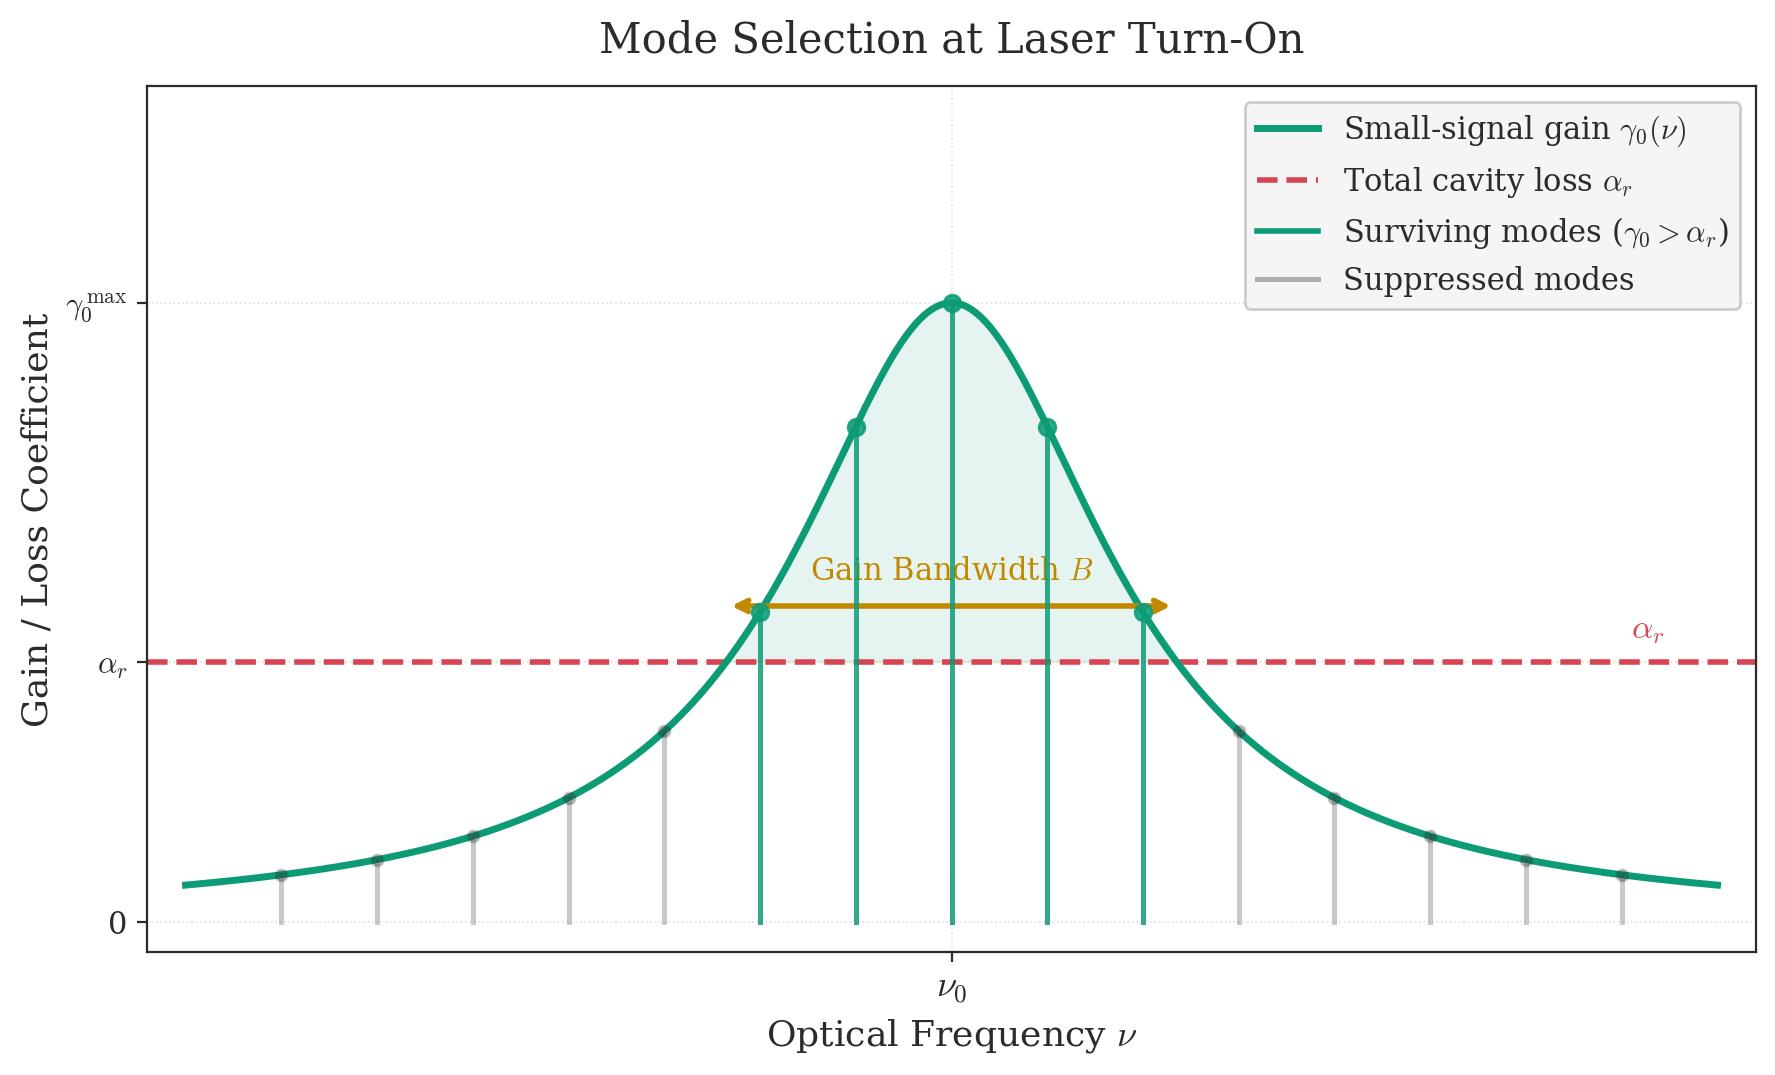
\includegraphics[width=0.6\textwidth]{Figures/Chapter 4/mode_selection_at_turnon.jpg}
    \caption{Mode Selection at Laser Turn-On: The Lorentzian small-signal gain profile $\gamma_0(\nu)$ sits above the flat loss line $\alpha_r$ over a finite bandwidth $B$. Only discrete FSR modes (the vertical comb) that fall within $B$ satisfy $\gamma_0(\nu_q) > \alpha_r$ and are candidates for oscillation. Modes outside $B$ are immediately suppressed.}
\end{figure}

\subsection{Homogeneous Broadening --- Global Saturation and Single-Mode Survival}

In a homogeneously broadened medium, all atoms are spectrally identical --- they all respond to the same optical field at every frequency. This means all modes compete for the same pool of inverted atoms. If one mode starts depleting the inversion, every other mode feels the gain drop.

As the dominant mode (the one closest to $\nu_0$) grows, its photon flux drives gain saturation uniformly across the whole lineshape. The saturated gain coefficient is:
\begin{equation*}
    \gamma(\nu, \Phi) = \frac{\gamma_0(\nu)}{1 + \Phi/\Phi_s}
\end{equation*}

The \emph{entire} gain curve is suppressed by the same factor $1/(1 + \Phi/\Phi_s)$. As the dominant mode saturates the gain down to $\alpha_r$ at its frequency, the gain at all other frequencies is also reduced below $\alpha_r$ and those modes die. The system eventually selects a single lasing mode.

\begin{keyinsight}[Homogeneous Broadening Leads to Single-Mode Lasing]
    In an ideally homogeneously broadened medium (ignoring spatial hole burning), gain saturation is \emph{global}: every mode competes for the same atoms. The mode with the highest small-signal gain wins, and all other modes die at steady state. The result is a single lasing mode at the frequency $\nu_q$ closest to the atomic resonance $\nu_0$.
\end{keyinsight}

\begin{figure}[H]
    \centering
    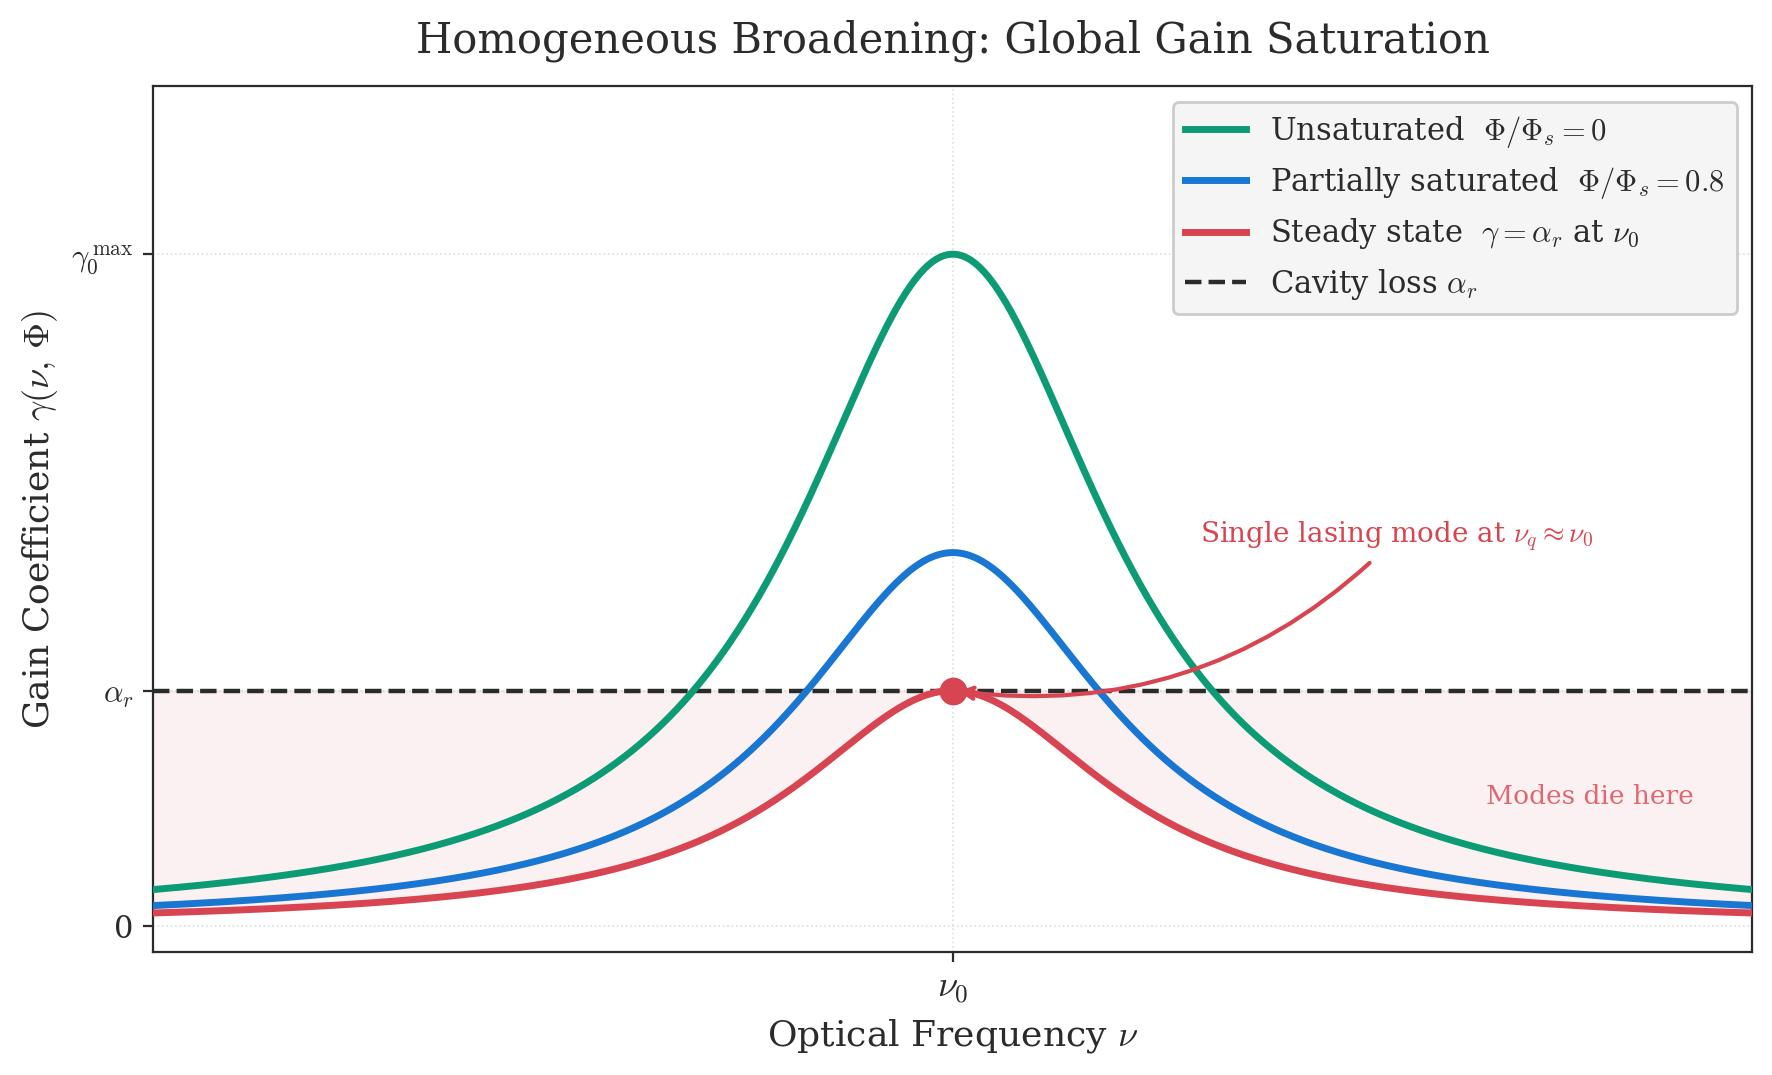
\includegraphics[width=0.6\textwidth]{Figures/Chapter 4/homogeneous_global_saturation.jpg}
    \caption{Homogeneous Broadening --- Global Gain Saturation: As the dominant mode near $\nu_0$ builds up photon flux, the entire Lorentzian gain curve sinks uniformly by the same suppression factor $1/(1+\Phi/\Phi_s)$. At steady state the gain touches $\alpha_r$ only at the winning mode frequency, driving the gain at all other mode frequencies below $\alpha_r$ simultaneously. All competing modes die.}
\end{figure}

\subsection{Spatial Hole Burning}

The homogeneous-versus-inhomogeneous distinction describes saturation in frequency space, but a standing-wave cavity also has structure in real space. The counter-propagating beams form an intensity pattern that alternates between peaks and nulls with period $\lambda/2$ along the cavity axis. Gain saturation is therefore not spatially uniform: it is strong at the intensity peaks and weak near the nulls. This is called \textbf{spatial hole burning}.

This effect is especially important because it weakens the ideal single-mode conclusion for homogeneously broadened media. A second longitudinal mode whose standing-wave peaks fall near the unsaturated regions left by the first mode can still find gain and survive. In other words, homogeneous broadening tries to enforce global mode competition, but spatial hole burning can reopen enough unsaturated gain for multiple modes to coexist.

\subsection{Inhomogeneous Broadening --- Spectral Hole Burning and \texorpdfstring{$\sqrt{\cdot}$}{Square-Root}-Saturation}

In an inhomogeneously broadened medium --- such as a Doppler-broadened gas laser --- different sub-groups of atoms resonate at different frequencies. A mode at $\nu_q$ interacts with those atoms whose resonance frequency is close to $\nu_q$ and does \emph{not} significantly perturb atoms resonant at other frequencies. Gain saturation is therefore \emph{local} in the frequency domain: as mode $\nu_q$ grows, it burns a narrow spectral hole in the gain profile --- depleting the inversion only of the atoms it resonates with, leaving the gain at other frequencies relatively untouched. This phenomenon is called \textbf{spectral hole burning}.

The key lies in understanding how each mode saturates its own private sub-group of atoms. A mode at frequency $\nu_q$ interacts only with those atoms whose resonance frequency matches $\nu_q$ --- the sub-group drawn from the narrow Lorentzian window of width $\Delta\nu_H$ centred at $\nu_q$. The local saturated gain for that sub-group follows the homogeneous saturation law, but the strong intracavity field simultaneously \textbf{power-broadens} the Lorentzian linewidth:
\begin{equation*}
    \Delta\nu_s = \Delta\nu_H\sqrt{1 + \Phi/\Phi_s}
\end{equation*}
This broadening matters. As $\Phi$ grows, the width $\Delta\nu_s$ grows with it, which means the mode can interact with a progressively wider band of atoms. Two competing effects are therefore at work simultaneously: the amplitude of the resonance is \emph{suppressed} by the factor $1/(1+\Phi/\Phi_s)$, but the \emph{width} of the resonance grows by $\sqrt{1+\Phi/\Phi_s}$. When the saturated lineshape is integrated over the atomic distribution to get the net gain, one power of $\sqrt{1+\Phi/\Phi_s}$ migrates from the width into the numerator and partially cancels the amplitude suppression in the denominator. The result is a weaker net saturation --- not the full $1/(1+\Phi/\Phi_s)$ of the homogeneous case, but only a square root:
\begin{keyresult}
    \begin{equation}
        \bar{\gamma}(\nu) = \frac{\gamma_0(\nu)}{\sqrt{1 + \Phi/\Phi_s}}
    \end{equation}
\end{keyresult}

where $\gamma_0(\nu)$ is the unsaturated (small-signal) gain at $\nu$, with the Gaussian (Doppler) spectral envelope.

This is the key structural difference from the homogeneous case. In homogeneous broadening, the saturated gain is $\gamma_0/(1+\Phi/\Phi_s)$ --- a full suppression factor. In inhomogeneous broadening, it is $\gamma_0/\sqrt{1+\Phi/\Phi_s}$ --- only a square root. The physical mechanism behind this difference is transparent from the derivation: saturation broadens the Lorentzian hole by $\sqrt{1+\Phi/\Phi_s}$ as the flux grows. This broadening introduces one power of $\sqrt{1+\Phi/\Phi_s}$ into the numerator through $\Delta\nu_s$, which then partially cancels the amplitude suppression in the denominator. The hole gets deeper but also wider; the two effects do not fully cancel, leaving a net $1/\sqrt{1+\Phi/\Phi_s}$.

The consequence for multi-mode behaviour is profound. In an IHB medium, different modes interact with different sub-groups of atoms, so their saturations are independent. Burning a hole at $\nu_q$ does not affect the gain available at $\nu_{q+1}$. Each mode can therefore coexist with all others, each depleting its own private pool of resonant atoms. IHB lasers natively support multi-mode oscillation, with the number of modes approximately equal to $B/\nu_F$. This contrasts sharply with the homogeneous case, where global saturation forces single-mode operation.

\begin{figure}[H]
    \centering
    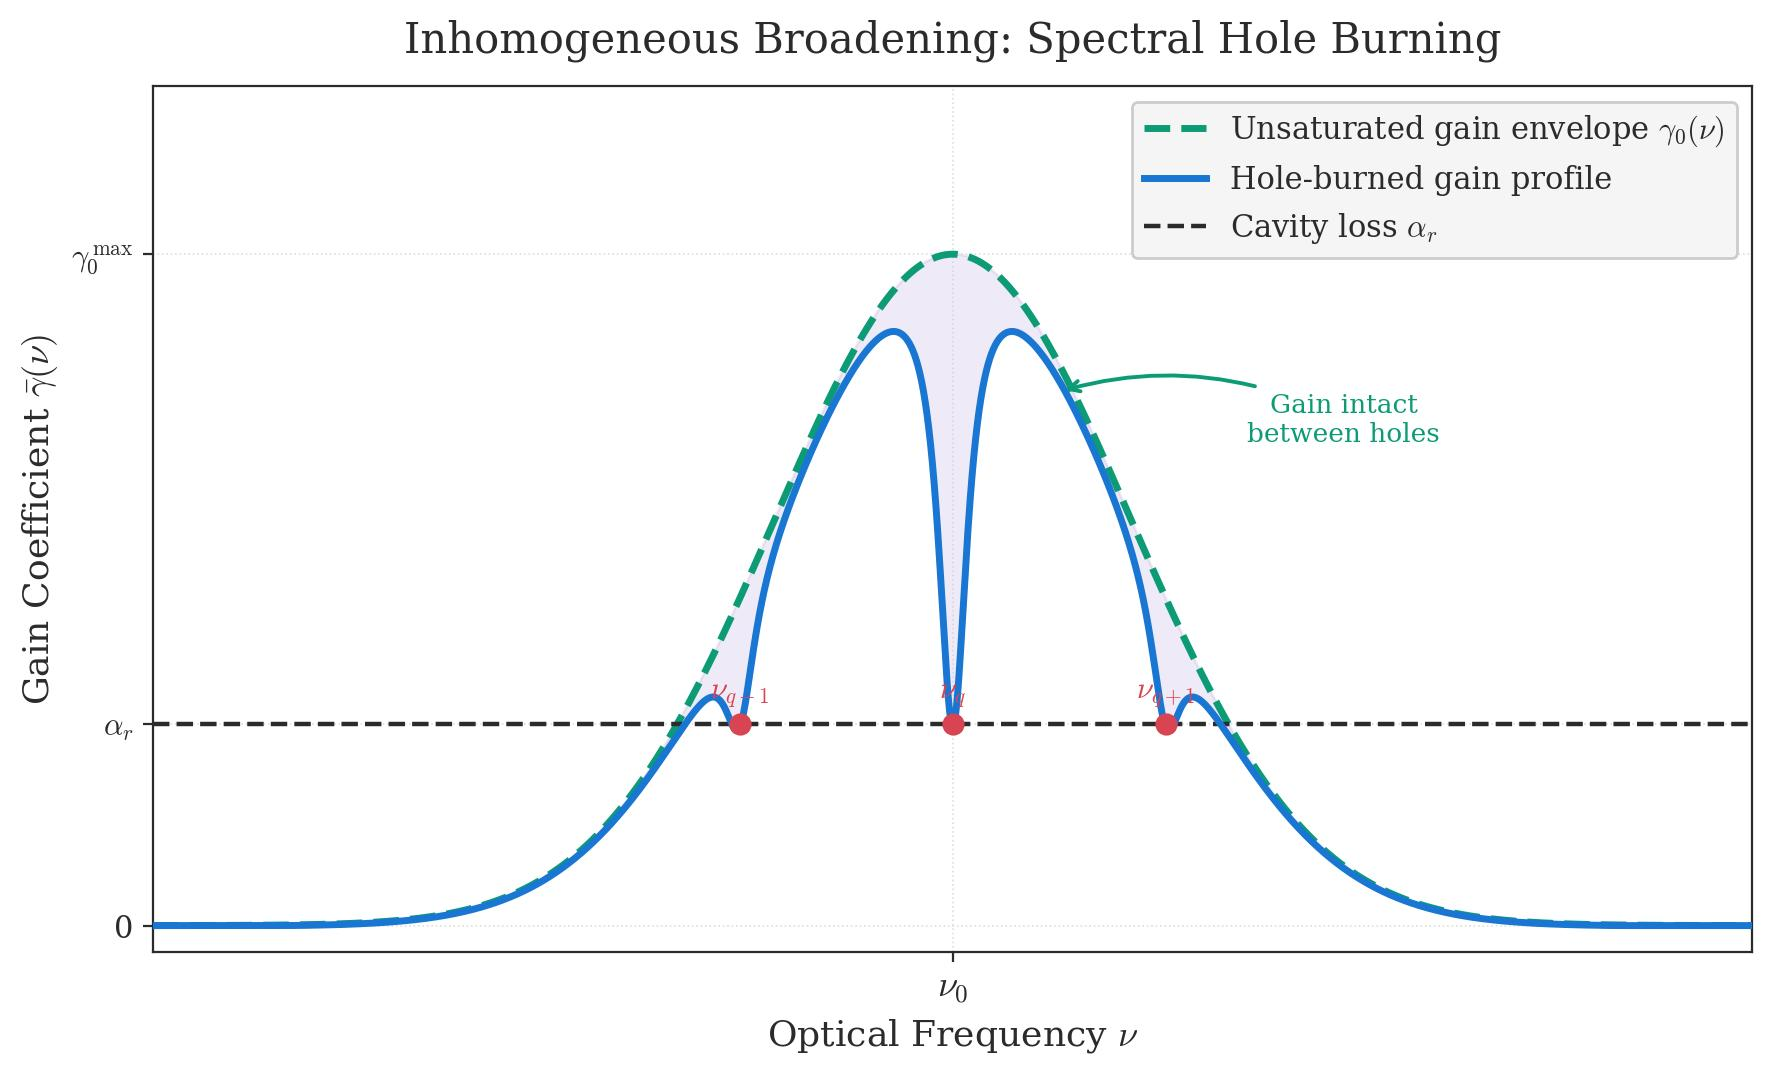
\includegraphics[width=0.6\textwidth]{Figures/Chapter 4/ihb_spectral_hole_burning.jpg}
    \caption{Inhomogeneous Broadening --- Spectral Hole Burning: Each lasing mode burns a narrow Lorentzian hole only into its local sub-group of resonant atoms. The broad Gaussian envelope (the unsaturated profile) remains largely intact between holes. Multiple modes therefore coexist independently, each depleting its own private pool of inverted atoms.}
\end{figure}

\begin{figure}[H]
    \centering
    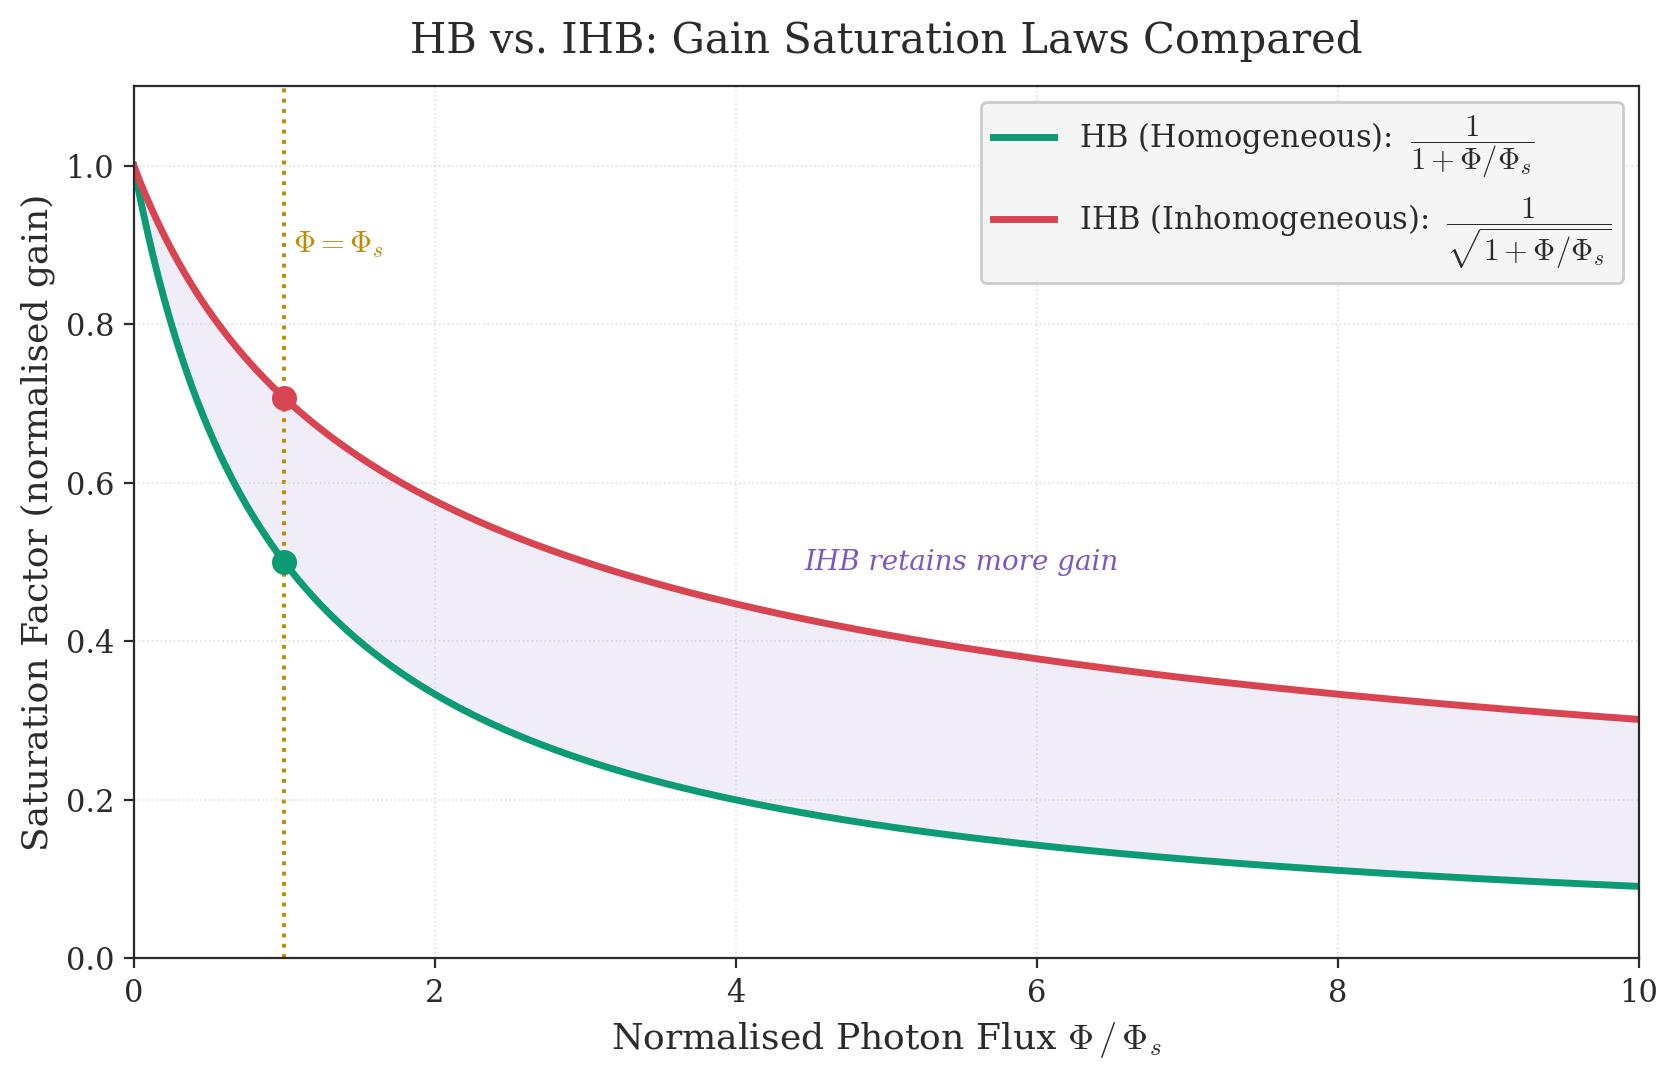
\includegraphics[width=0.6\textwidth]{Figures/Chapter 4/hb_vs_ihb_saturation_law.jpg}
    \caption{HB vs.\ IHB Saturation Laws: A homogeneously broadened medium saturates as $1/(1+\Phi/\Phi_s)$, while an inhomogeneously broadened medium saturates far more slowly as $1/\sqrt{1+\Phi/\Phi_s}$. The shaded region between the curves represents the additional gain retained by the IHB medium at the same photon flux --- the direct reason IHB lasers accumulate higher intracavity power and support multi-mode oscillation.}
\end{figure}

\subsection{The Lamb Dip (Doppler Medium)}

The general IHB picture applies to any inhomogeneously broadened medium. But in a gas laser --- the canonical IHB system --- the inhomogeneous broadening arises from the thermal motion of atoms, and the resulting Doppler picture has an important subtlety worth examining explicitly.

Consider an atom moving with velocity $v$ along the cavity axis. Because of the Doppler effect, this atom does not interact with light at $\nu_0$ but at a shifted frequency. An atom moving \emph{toward} the incoming beam sees it blue-shifted to $\nu_0(1 + v/c)$; an atom moving \emph{away} sees it red-shifted to $\nu_0(1 - v/c)$.

The intracavity mode at frequency $\nu_q$ is a standing wave --- the superposition of two counter-propagating beams. This means a single mode at $\nu_q$ resonates simultaneously with \emph{two} distinct velocity classes:
\begin{itemize}
    \item Atoms moving toward the rightward beam with speed $+v$ such that $\nu_q = \nu_0(1 + v/c)$.
    \item Atoms moving toward the leftward beam with speed $-v$ such that $\nu_q = \nu_0(1 - v/c)$, i.e.\ the same speed magnitude $|v| = c|\nu_q/\nu_0 - 1|$.
\end{itemize}
The mode therefore saturates atoms on \emph{both} sides of the Doppler distribution, burning \emph{two} symmetric spectral holes --- one on each side of the central frequency $\nu_0$.

As the mode frequency $\nu_q$ is tuned toward line centre $\nu_0$ and eventually reaches $\nu_q = \nu_0$, the two velocity classes merge: both the $+v$ and $-v$ groups collapse to $v = 0$. Instead of drawing from two separate pools, the mode now draws from a single, shared pool of stationary atoms. The number of active atoms available to the mode therefore \emph{decreases} as $\nu_q \to \nu_0$, even though the unsaturated gain is highest at line centre.

This causes the mode output power to actually \emph{decrease} as $\nu_q$ is tuned through $\nu_0$. The output power as a function of $\nu_q$ traces a bell-curve with a central \textbf{depression} at line centre. This central dip is called the \textbf{Lamb dip}.

\begin{keyinsight}[The Lamb Dip]
    In a Doppler-broadened medium, a mode at $\nu_q \neq \nu_0$ burns two holes simultaneously in the gain profile --- one for each velocity class resonating with the standing-wave field. When $\nu_q = \nu_0$, the two holes collapse into one because only the $v = 0$ atoms are available. The mode loses half its pool of active atoms, and the power drops. The resulting central depression in the mode's frequency-tuning curve is the \textbf{Lamb dip} --- a direct signature of the two-hole burning mechanism unique to standing-wave cavities in Doppler-broadened media.
\end{keyinsight}

\begin{figure}[H]
    \centering
    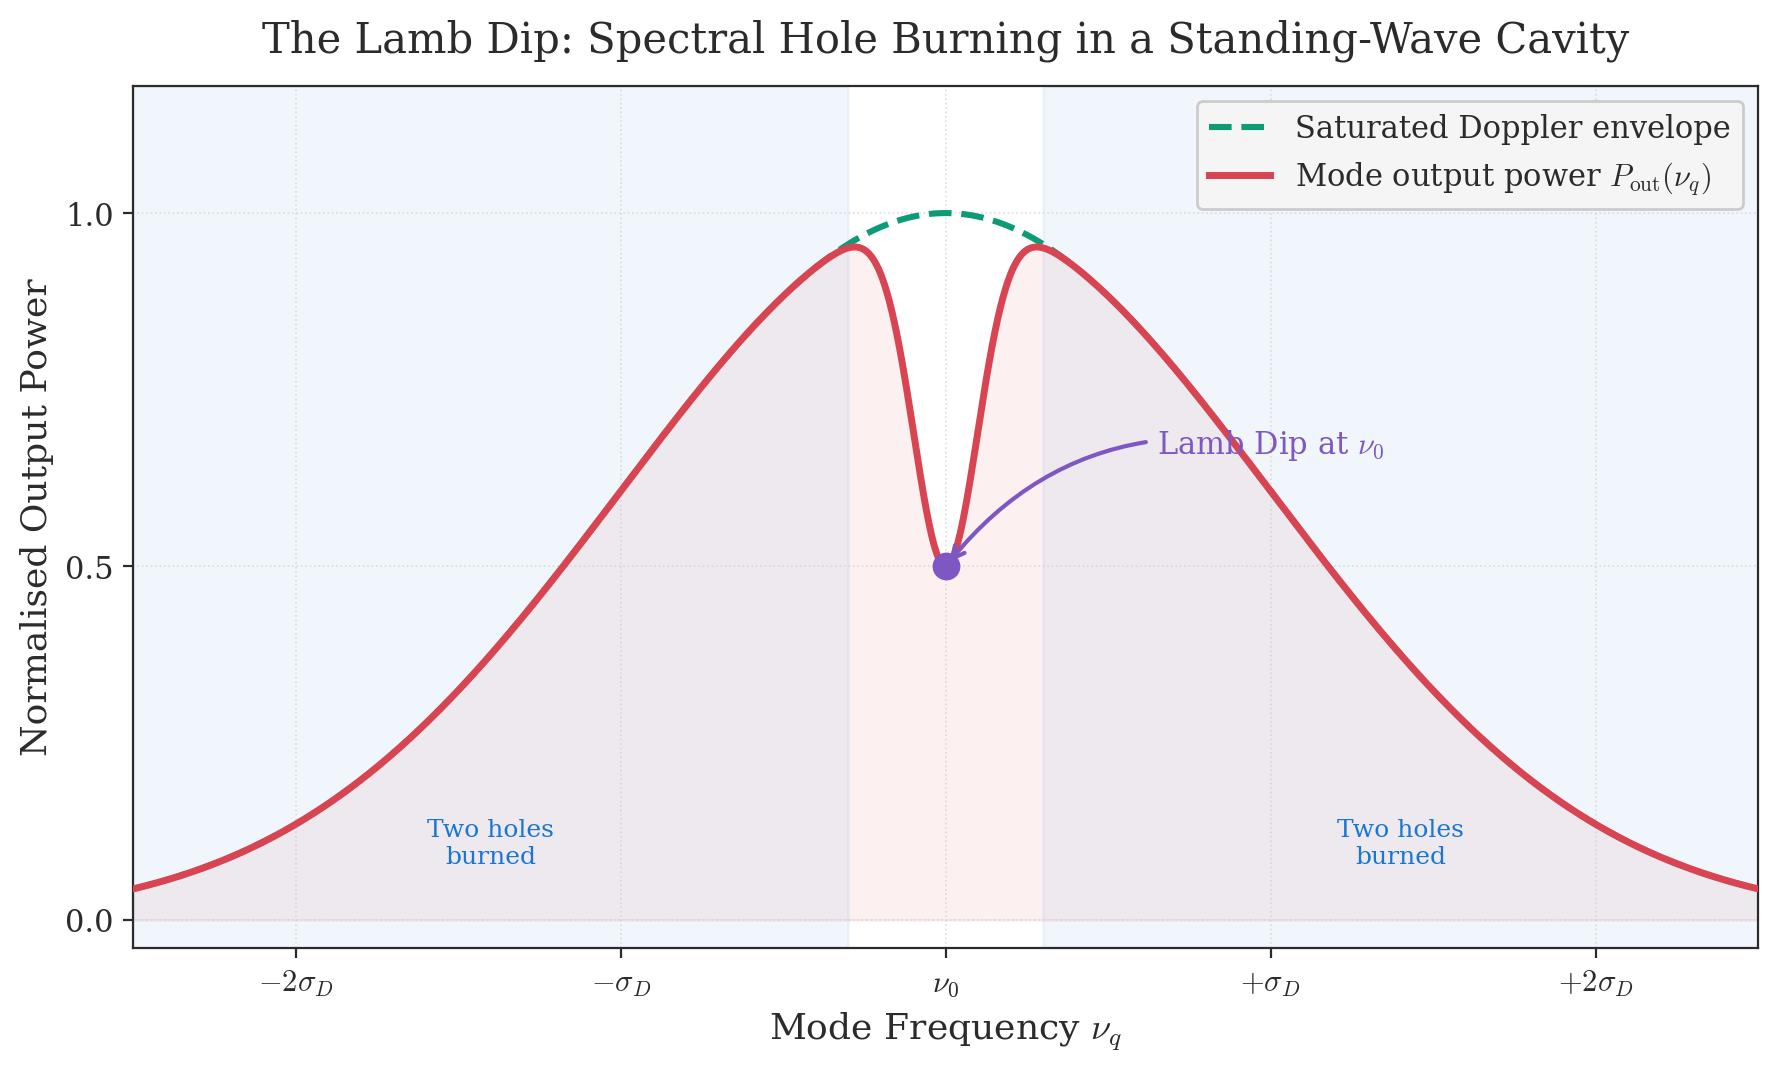
\includegraphics[width=0.6\textwidth]{Figures/Chapter 4/lamb_dip.jpg}
    \caption{The Lamb Dip: Output power of a Doppler-broadened laser as a function of the mode frequency $\nu_q$. Away from line centre the mode simultaneously burns two spectral holes (one per velocity class resonating with each counter-propagating beam), drawing from two pools of atoms. At $\nu_q = \nu_0$ the two velocity classes collapse to $v = 0$ and the mode draws from a single shared pool --- the available gain drops, and the output power dips. The narrow central depression is the Lamb dip.}
\end{figure}

\begin{figure}[H]
    \centering
    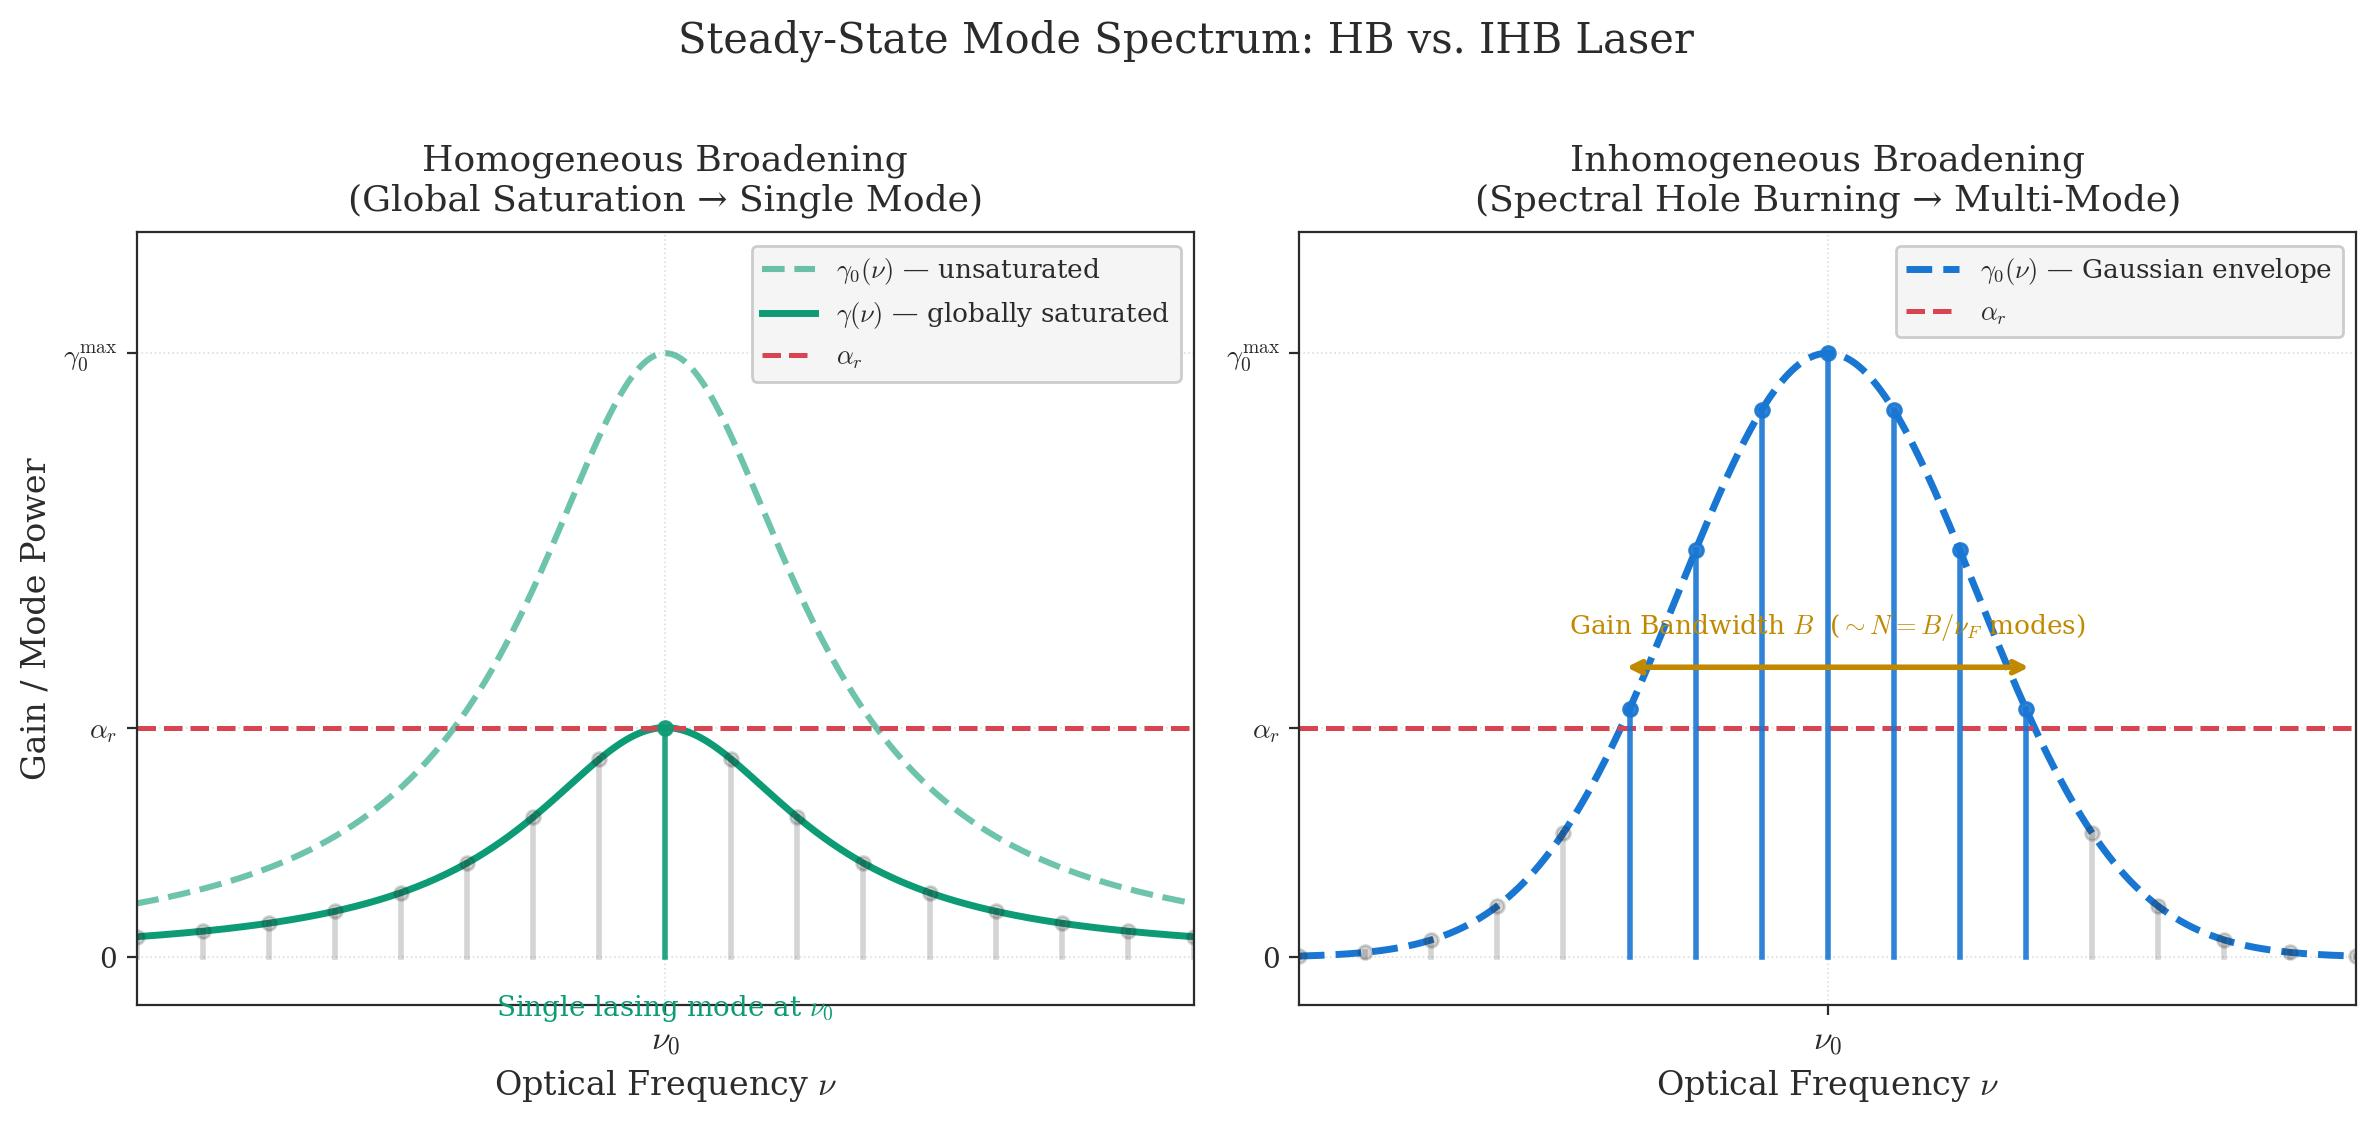
\includegraphics[width=0.8\textwidth]{Figures/Chapter 4/hb_vs_ihb_mode_spectrum.jpg}
    \caption{Steady-State Mode Spectrum --- HB vs.\ IHB Laser: In the homogeneously broadened case (left), global gain saturation suppresses the entire Lorentzian uniformly until the strongest cavity mode just touches $\alpha_r$, leaving only one surviving longitudinal mode. In the inhomogeneously broadened case (right), each mode burns its own independent spectral hole and does not affect others; all modes within the gain bandwidth $B$ survive simultaneously, producing a rich multi-mode output spectrum.}
\end{figure}

With the steady-state mode structure fully understood --- which modes survive, how many there are, and why the broadening mechanism is the deciding factor --- we can now calculate how much optical power the laser actually delivers.


% ----------------------------------------------------------
%  Part C: Steady-State Output Power
% ----------------------------------------------------------
With the qualitative mechanics of mode survival and the physical laws of spectral saturation fully established, we can now translate these homogeneous and inhomogeneous saturation profiles into quantitative equations for the laser's steady-state output power and derive how to optimize its mirrors for maximum efficiency.

\subsection{Homogeneously Broadened Laser: Steady-State Intracavity Photon-Flux Density}

At steady state, gain saturation has driven the gain exactly to the loss level: $\gamma = \alpha_r$. For a homogeneously broadened medium:
\begin{equation*}
    \frac{\gamma_0}{1 + \Phi/\Phi_s} = \alpha_r
\end{equation*}

Solving for the intracavity photon-flux density $\Phi$:
\begin{equation*}
    1 + \frac{\Phi}{\Phi_s} = \frac{\gamma_0}{\alpha_r}
    \quad\Longrightarrow\quad
    \frac{\Phi}{\Phi_s} = \frac{\gamma_0}{\alpha_r} - 1
\end{equation*}
\begin{keyresult}
    \begin{equation}
        \Phi = \Phi_s\!\left(\frac{\gamma_0}{\alpha_r} - 1\right), \qquad \gamma_0 > \alpha_r
    \end{equation}
\end{keyresult}

and $\Phi = 0$ if $\gamma_0 \leq \alpha_r$ (below threshold, no oscillation). The intracavity photon flux represents photons travelling in both directions; for a symmetric cavity ($R_1 = R_2$) the flux in each direction is approximately $\Phi/2$.

\begin{figure}[H]
    \centering
    
\includegraphics[width=0.6\textwidth]{Figures/Chapter 4/gain_saturation_curve.jpg}
    \caption{Gain Clamping at Threshold: Below threshold the small-signal gain $\gamma_0$ rises linearly with pump rate while the intracavity flux remains zero. Once the pump crosses $R_\mathrm{th}$, oscillation begins and gain saturation clamps $\gamma$ exactly to $\alpha_r$ regardless of further pumping. The excess pump energy instead drives exponential growth in the intracavity photon flux $\Phi/\Phi_s$ (right axis).}
\end{figure}

\subsection{Output Power Through a Mirror}

The output power through mirror $M_1$ with power transmission $T_1 = 1 - R_1$ is:
\begin{equation*}
    P_{\text{out},1} = \frac{\Phi}{2}\cdot h\nu\cdot A\cdot T_1
\end{equation*}
where $A$ is the cross-sectional beam area and the factor $1/2$ accounts for only the forward-travelling flux exiting through $M_1$. Substituting the steady-state flux:
\begin{equation*}
    P_{\text{out},1} = \frac{\Phi_s}{2}\cdot h\nu\cdot A\cdot T_1 \cdot\left(\frac{\gamma_0}{\alpha_r} - 1\right)
\end{equation*}

Defining $P_s = \Phi_s\,h\nu\,A$ as the \textbf{saturation power:}
\begin{equation*}
    P_{\text{out},1} = \frac{P_s}{2}\,T_1\!\left(\frac{\gamma_0}{\alpha_r} - 1\right)
\end{equation*}

For a symmetric cavity ($R_1 = R_2 = R$, $T = 1 - R$) with low transmissivity ($T \ll 1$) we approximate $\ln(1/R) \approx T$ and:
\begin{equation*}
    \alpha_r \approx \alpha_s + \frac{T}{L}
\end{equation*}

Defining the round-trip gain $g = 2\gamma_0 L$ and round-trip internal loss $\ell = 2\alpha_s L$:
\begin{equation*}
    \frac{\gamma_0}{\alpha_r} \approx \frac{g/2L}{(\ell/2L) + (T/L)} = \frac{g}{\ell + T}
\end{equation*}
\begin{keyresult}
    \begin{equation}
        P_{\text{out}} = \frac{P_s}{2}\cdot T\!\left(\frac{g}{\ell + T} - 1\right)
        = \frac{P_s}{2}\cdot\frac{T(g - \ell - T)}{\ell + T}
    \end{equation}
\end{keyresult}

\subsection{Optimal Mirror Transmission and Maximum Output Power}

We can notice that the output power depends on the mirror transmissivity $T$. There is clearly a tension: if $T$ is too small, very little light exits even though the intracavity power is high; if $T$ is too large, the loss is so great that the gain barely exceeds threshold and the power is again small. An optimal transmissivity $T_{\text{opt}}$ must therefore exist.

We differentiate the output power with respect to $T$ and set the derivative to zero:
\begin{equation*}
    \frac{dP_{\text{out}}}{dT}
    = \frac{P_s}{2}\!\left[\frac{g(\ell + T) - gT}{(\ell + T)^2} - 1\right]
    = \frac{P_s}{2}\!\left[\frac{g\ell}{(\ell + T)^2} - 1\right] = 0
\end{equation*}

Setting the bracket to zero and solving for $T_{\text{opt}}$:
\begin{equation*}
    \frac{g\ell}{(\ell + T_{\text{opt}})^2} = 1
    \quad\Longrightarrow\quad
    \ell + T_{\text{opt}} = \sqrt{g\ell}
\end{equation*}
\begin{keyresult}
    \begin{equation}
        T_{\text{opt}} = \sqrt{g\ell} - \ell
    \end{equation}
\end{keyresult}

Substituting $T_{\text{opt}}$ back, at $T = T_{\text{opt}}$:
\begin{equation*}
    \frac{g}{\ell + T_{\text{opt}}} - 1 = \frac{g}{\sqrt{g\ell}} - 1 = \sqrt{\frac{g}{\ell}} - 1
    = \frac{\sqrt{g} - \sqrt{\ell}}{\sqrt{\ell}}
\end{equation*}

So:
\begin{equation*}
    P_{\text{max}}
    = \frac{P_s}{2}\cdot(\sqrt{g\ell} - \ell)\cdot\frac{\sqrt{g} - \sqrt{\ell}}{\sqrt{\ell}}
    = \frac{P_s}{2}\cdot\sqrt{\ell}(\sqrt{g} - \sqrt{\ell})\cdot\frac{\sqrt{g} - \sqrt{\ell}}{\sqrt{\ell}}
\end{equation*}
\begin{keyresult}
    \begin{equation}
        P_{\text{max}} = \frac{P_s}{2}\!\left(\sqrt{g} - \sqrt{\ell}\right)^{\!2}
    \end{equation}
\end{keyresult}

\begin{keyinsight}[Maximum Laser Output Power]
    The maximum output power $P_{\text{max}} = \frac{P_s}{2}(\sqrt{g} - \sqrt{\ell})^2$ is achieved at the optimal transmissivity $T_{\text{opt}} = \sqrt{g\ell} - \ell$. The $({\sqrt{g} - \sqrt{\ell}})^2$ structure reveals a fundamental trade-off: as the gain $g$ increases above the loss $\ell$, the maximum achievable power grows quadratically with the excess. At threshold ($g = \ell$), $P_{\text{max}} = 0$ --- no output power is produced. There is also a trade-off in choosing $T$: perfect mirrors ($T = 0$) trap all the light inside and produce zero output, while too high a $T$ raises the threshold so much that little inversion is left to drive the oscillation. The optimum balances both effects.
\end{keyinsight}

\begin{figure}[H]
    \centering
    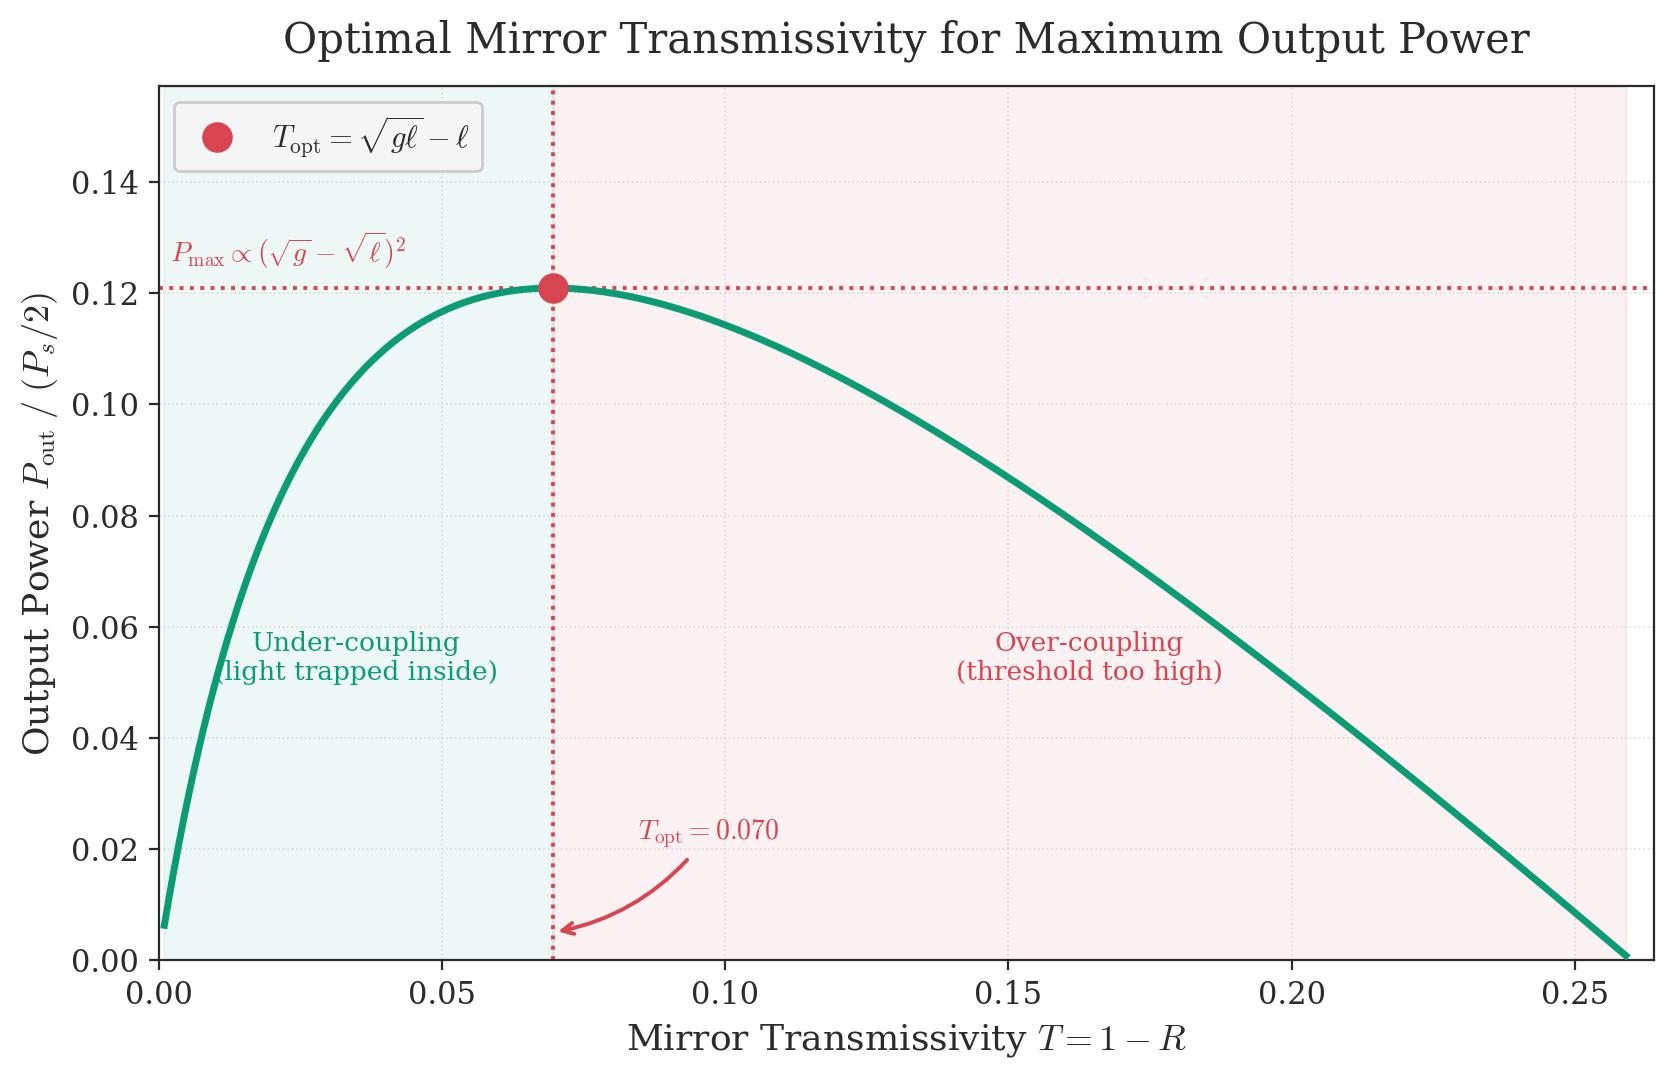
\includegraphics[width=0.6\textwidth]{Figures/Chapter 4/output_power_vs_transmission.jpg}
    \caption{Optimal Mirror Transmissivity: Output power $P_\mathrm{out}$ as a function of mirror transmissivity $T$. In the under-coupling regime ($T < T_\mathrm{opt}$) most photons are trapped inside the cavity and little power exits. In the over-coupling regime ($T > T_\mathrm{opt}$) the round-trip loss exceeds the gain so severely that the intracavity power collapses. The maximum $P_\mathrm{max} \propto (\sqrt{g}-\sqrt{\ell})^2$ is reached at the unique optimal transmissivity $T_\mathrm{opt} = \sqrt{g\ell} - \ell$.}
\end{figure}

\subsection{Inhomogeneously Broadened Laser: Steady-State Power}

All of the output-power analysis above assumed a homogeneously broadened medium. For an inhomogeneously broadened laser the saturated gain takes the square-root form, but at steady state the gain must still lock exactly to the loss. Setting $\bar{\gamma} = \alpha_r$:
\begin{equation*}
    \frac{\gamma_0}{\sqrt{1 + \Phi_m/\Phi_s}} = \alpha_r
\end{equation*}
where $\Phi_m$ is the steady-state intracavity photon flux. Solving step by step --- first isolate the square root:
\begin{equation*}
    \sqrt{1 + \frac{\Phi_m}{\Phi_s}} = \frac{\gamma_0}{\alpha_r}
\end{equation*}
Squaring both sides:
\begin{equation*}
    1 + \frac{\Phi_m}{\Phi_s} = \left(\frac{\gamma_0}{\alpha_r}\right)^{\!2}
    \quad\Longrightarrow\quad
    \frac{\Phi_m}{\Phi_s} = \left(\frac{\gamma_0}{\alpha_r}\right)^{\!2} - 1
\end{equation*}
Multiplying through by $P_s = \Phi_s\,h\nu\,A$ to convert to power:
\begin{keyresult}
    \begin{equation}
        P_m = P_s\!\left[\left(\frac{\gamma_0}{\alpha_r}\right)^{\!2} - 1\right]
    \end{equation}
\end{keyresult}
where $P_m$ is the steady-state intracavity power. Comparing this to the HB result $P = P_s(\gamma_0/\alpha_r - 1)$, we can factor the IHB result as:
\begin{equation*}
    P_m = P_s\!\left(\frac{\gamma_0}{\alpha_r} + 1\right)\!\left(\frac{\gamma_0}{\alpha_r} - 1\right)
\end{equation*}
The extra factor $(\gamma_0/\alpha_r + 1) > 1$ means the IHB laser accumulates \emph{more} intracavity power for the same pump level above threshold compared to the HB laser. This is a direct consequence of the weaker square-root saturation: gain does not collapse as quickly, so more photons build up before equilibrium is reached.

\subsubsection*{Power Variation Across Modes in an Inhomogeneously Broadened Laser}

In the preceding subsection we computed the total intracavity power for a single dominant mode evaluated at the gain peak. In a multi-mode IHB laser, however, each mode at frequency $\nu_q$ sits at a different point on the Gaussian gain envelope, so it sees its own individual small-signal gain:
\begin{equation*}
    \gamma_0(\nu_q) = \gamma_{0,\max}\,\exp\!\left(-\frac{(\nu_q - \nu_0)^2}{2\sigma_D^2}\right)
\end{equation*}

Since IHB modes saturate independently through their own private pool of resonant atoms, we apply the square-root steady-state condition mode by mode. For each mode $q$, setting its saturated gain equal to $\alpha_r$:
\begin{equation*}
    \frac{\gamma_0(\nu_q)}{\sqrt{1 + \Phi_q/\Phi_s}} = \alpha_r
    \quad\Longrightarrow\quad
    \frac{\Phi_q}{\Phi_s} = \left(\frac{\gamma_0(\nu_q)}{\alpha_r}\right)^{\!2} - 1
\end{equation*}

The output power from mode $q$ through a mirror of transmissivity $T$ is therefore proportional to $\Phi_q$:
\begin{equation*}
    P_q \propto P_s\!\left[\left(\frac{\gamma_0(\nu_q)}{\alpha_r}\right)^{\!2} - 1\right]
\end{equation*}

The physical message is clear. Modes near the centre of the gain profile ($\nu_q \approx \nu_0$) have a high $\gamma_0(\nu_q)$ and accumulate the most intracavity photons, producing the highest output power. Modes near the edges of the lasing bandwidth have $\gamma_0(\nu_q)$ only slightly above $\alpha_r$, so $(\gamma_0/\alpha_r)^2 \approx 1$ and their contribution is negligible. The multi-mode output spectrum of an IHB laser is therefore not a flat frequency comb --- it is a structured set of lines whose envelope mimics the squared gain profile, peaked at $\nu_0$ and decaying to zero at both sides of the gain bandwidth $B$.

\begin{keyinsight}[IHB Laser Output Is Not a Flat Comb]
    A common misconception is that an IHB laser's multi-mode output is a flat frequency comb because all modes survive simultaneously. In reality, the per-mode output power varies dramatically across the spectrum. Modes closest to the atomic resonance $\nu_0$ enjoy the highest gain, saturate hardest, and dominate the output. Edge modes barely exceed threshold and emit very little power. The envelope of the output spectrum is a Gaussian-shaped curve (inheriting the Doppler gain profile), not a rectangular window.
\end{keyinsight}

% ----------------------------------------------------------
%  Section 3: The Fabry-P\'{e}rot Resonator
% ----------------------------------------------------------
\section{The Fabry-P\'{e}rot Resonator}

The round-trip conditions derived in the first section define \emph{when} the Fabry-P\'{e}rot cavity will cross the threshold into self-sustained oscillation. They do not, however, tell us \emph{how sharply} the cavity filters its resonant modes, or \emph{how a signal is amplified} when the gain falls short of the threshold (the sub-threshold regime).

To build a complete electromagnetic wave description of the cavity, we must step back from the running oscillator and study the formal filter theory of the resonator. This derivation gives the mode linewidth, the Airy spectrum, and the finesse their precise physical and mathematical foundations. Crucially, by then switching on sub-threshold gain, we recover the Fabry-P\'{e}rot amplifier response and show that as its gain approaches the threshold derived in \S1.2, the amplifier's response diverges to infinity --- beautifully recovering the laser oscillator as a natural, continuous limiting case of a sub-threshold amplifier.

This section has two halves. We first study the \emph{cold} passive cavity, where the mirrors alone create the Airy spectrum, the free spectral range, and the linewidth. We then switch on sub-threshold gain and recover the Fabry-P\'{e}rot amplifier response, whose limiting case is exactly laser oscillation.

\subsection{The Passive Cavity}
\subsubsection{Three operating regimes}

The operating point of a Fabry-P\'{e}rot device is fully specified by comparing the gain inside the cavity with the total cavity loss $\alpha_r$ we derived above:

\begin{itemize}
    \item If $\gamma = 0$, the cavity is a \textbf{passive resonator}. It does not amplify light; it only filters frequency by storing resonant fields longer than non-resonant fields.
    \item If $0 < \gamma_{ss} < \alpha_r$, the round-trip gain is still less than the round-trip loss. The field cannot self-sustain, but an injected signal is selectively amplified --- this is the \textbf{FP amplifier} regime.
    \item If $\gamma_{ss} \geq \alpha_r$, round-trip gain reaches or exceeds round-trip loss. The field can grow without an injected signal, and gain saturation then clamps the steady-state gain to $\alpha_r$ --- this is the \textbf{laser oscillator} regime.
\end{itemize}

The connection to the travelling-wave amplifier (TWA) is direct: forcing $R_1 = R_2 = 0$ makes $\alpha_r \to \infty$, so $\gamma_{ss} < \alpha_r$ is trivially satisfied for any finite gain --- which is exactly why the perfectly anti-reflected TWA can never oscillate.
\subsubsection{Passive cavity intensity spectrum --- the Airy function}

To derive the explicit cavity linewidth and gain spectrum, we first study the cold cavity ($\gamma = 0$) by summing all rightward-travelling field contributions. Every additional round trip multiplies the field by $r_1 r_2 e^{-j2\beta L}e^{-\alpha_s L}$, so the total forward field is an infinite geometric series:
\begin{equation*}
    E^{+} = E_0\!\left[1 + r_1 r_2 e^{-j2\beta L}e^{-\alpha_s L}
        + \!\left(r_1 r_2 e^{-j2\beta L}e^{-\alpha_s L}\right)^2 + \cdots\right]
\end{equation*}

The series converges (modulus $r_1 r_2 e^{-\alpha_s L} < 1$ for any lossy cavity) to:
\begin{equation}
    E^{+} = \frac{E_0}{1 - r_1 r_2\,e^{-j2\beta L}\,e^{-\alpha_s L}} \tag{I}
\end{equation}

The optical intensity $I^{+} = |E^{+}|^2/(2\eta)$ follows from multiplying \textup{(I)} by its complex conjugate. Using $e^{j\theta}+e^{-j\theta}=2\cos\theta$ then $\cos\theta = 1-2\sin^2(\theta/2)$, the denominator's constant terms collect into a perfect square:
\begin{equation*}
    I^{+} = \frac{|E_0|^2}{2\eta}\cdot
    \frac{1}{\left(1-r_1 r_2 e^{-\alpha_s L}\right)^2+4\,r_1 r_2 e^{-\alpha_s L}\sin^2(\beta L)}
\end{equation*}

This is the \textbf{Airy function} of the cavity --- it confirms the resonance frequencies we derived from the phase condition ($\sin(\beta L)=0$) and gives the exact lineshape. The half-power condition $I^+ = I^+_{\max}/2$ yields:
\begin{equation*}
    4\,r_1 r_2 e^{-\alpha_s L}\sin^2(\beta L) = \left(1 - r_1 r_2 e^{-\alpha_s L}\right)^2
\end{equation*}

Solving for $\sin(\beta L)$, substituting $\beta = 2\pi\nu/c$, doubling for the full FWHM, and writing $c/(2L) = \nu_F$:
\begin{equation*}
    \delta\nu = \frac{2\nu_F}{\pi}\,\sin^{-1}\!\left[\frac{1 - r_1 r_2 e^{-\alpha_s L}}{2\sqrt{r_1 r_2 e^{-\alpha_s L}}}\right]
\end{equation*}

\begin{figure}[H]
    \centering
    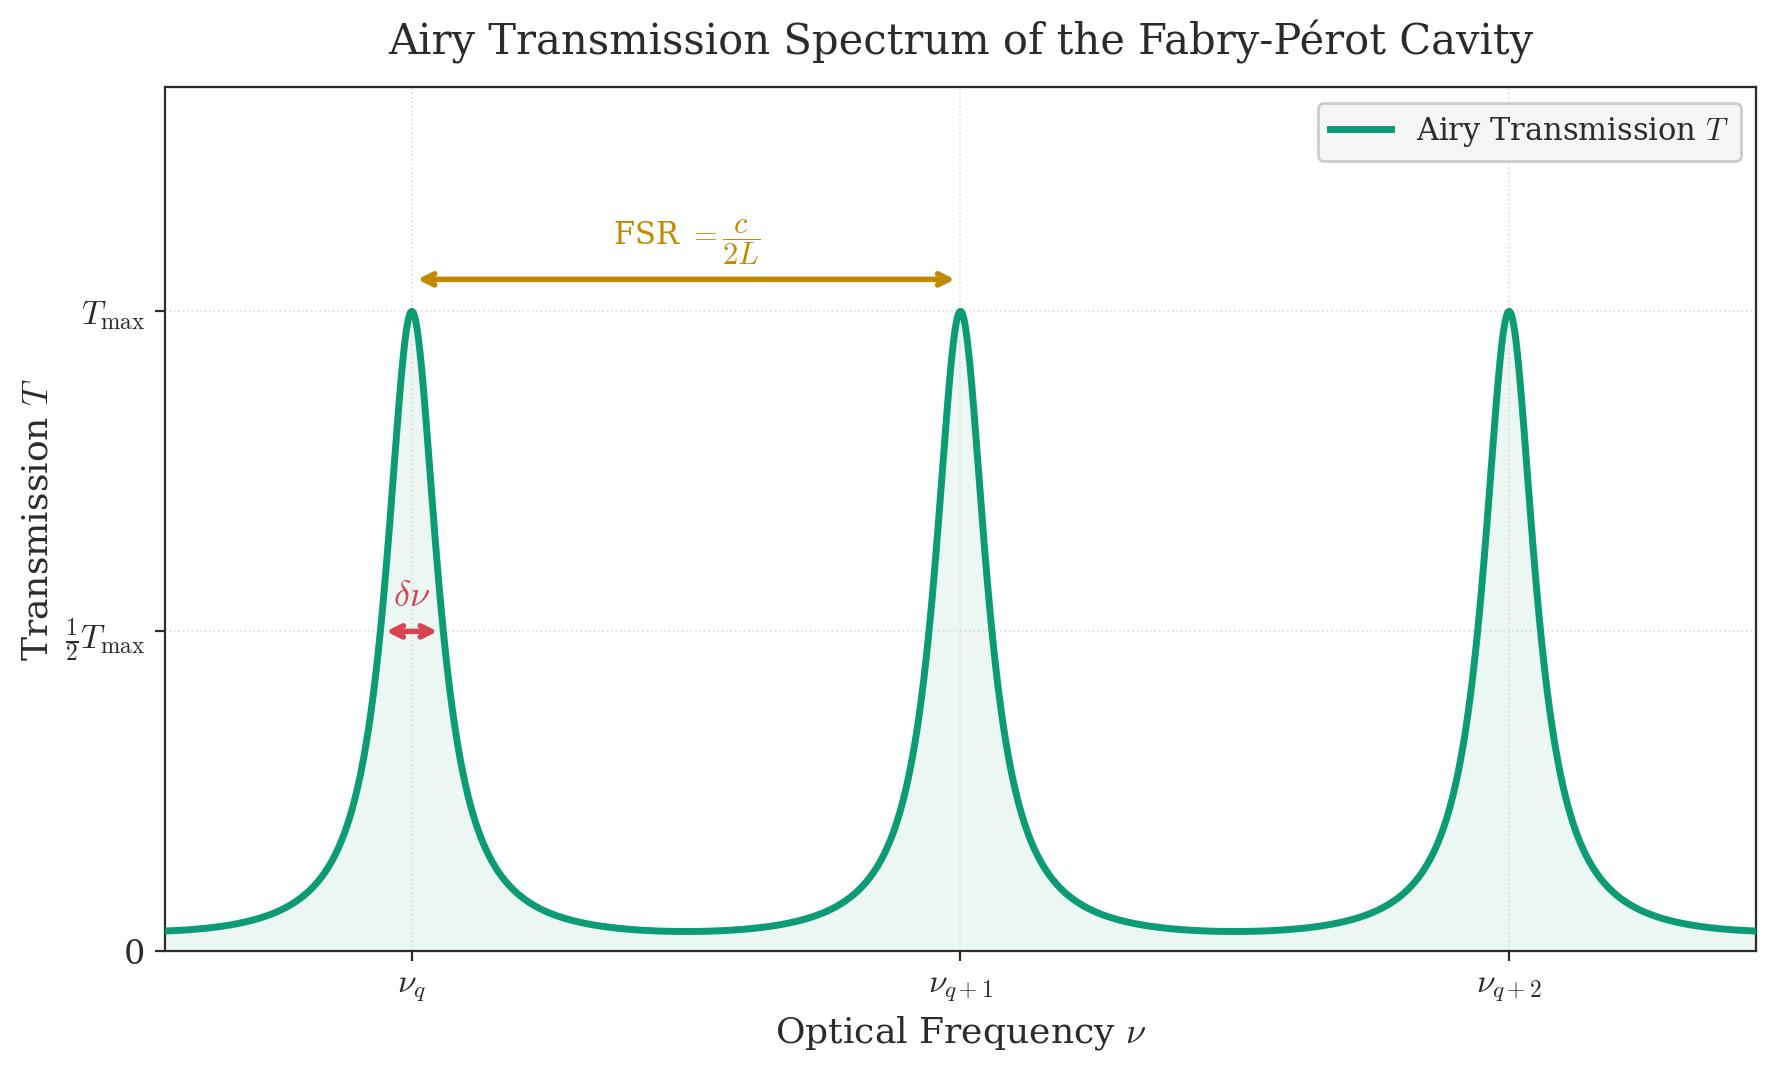
\includegraphics[width=0.6\textwidth]{Figures/Chapter 4/airy_function_spectrum.jpg}
    \caption{Passive Cavity Airy Spectrum: The intracavity intensity as a function of optical frequency forms a comb of sharp resonance peaks separated by the FSR $= c/2L$. The FWHM of each peak $\delta\nu$ and the finesse $\mathcal{F} = \mathrm{FSR}/\delta\nu$ are both set by the total round-trip loss $\alpha_r L$. As mirror reflectivity increases, the peaks sharpen and the finesse diverges.}
\end{figure}
\subsubsection{Free spectral range, mode linewidth, and finesse}

The resonance peaks of the Airy function occur whenever $\sin(\beta L) = 0$, i.e.\ when $\beta L = q\pi$ for integer $q$. Consecutive resonances are separated in frequency by:
\begin{keyresult}
    \begin{equation}
        \nu_F = \frac{c}{2L}
    \end{equation}
\end{keyresult}

This is the \textbf{Free Spectral Range} (FSR) --- the frequency spacing between adjacent longitudinal modes. The $q$-th mode sits at $\nu_q = q\,\nu_F$, recovering our cold-resonator result from the phase condition. The finesse is defined as the ratio of the FSR to the mode linewidth:
\begin{keyresult}
    \begin{equation}
        \mathcal{F} = \frac{\nu_F}{\delta\nu}
    \end{equation}
\end{keyresult}

The finesse plays the same role for a Fabry-P\'{e}rot resonator as the quality factor $Q$ does for an electronic resonator --- it quantifies how sharply the resonances are defined. For a high-finesse cavity, the small-angle approximation $\sin^{-1}(x) \approx x$ applies.

Depending on the cavity's loss characteristics, several key approximations for the finesse are widely used in practice:
\begin{enumerate}
    \item \textbf{Mirror-Limited Finesse (Lossless Cavity):} In an ideal cavity with zero internal medium loss ($\alpha_s = 0$) and identical mirrors ($R_1 = R_2 = R$), the finesse depends solely on the mirror reflectivities:
          \begin{keyresult}
              \begin{equation}
                  \mathcal{F} \approx \frac{\pi\sqrt{R}}{1 - R}
              \end{equation}
          \end{keyresult}
          This represents the upper mirror-limited bound of the cavity's resolving power.

    \item \textbf{Generalized Lossy Finesse:} Converting $r_i = \sqrt{R_i}$ in the full Airy half-power condition gives the explicit formula accounting for both unequal mirrors and internal medium scattering/absorption ($\alpha_s > 0$):
          \begin{keyresult}
              \begin{equation}
                  \mathcal{F} \approx \frac{\pi\,(R_1 R_2)^{1/4}\,e^{-\alpha_s L/2}}{1 - \sqrt{R_1 R_2}\,e^{-\alpha_s L}}
              \end{equation}
          \end{keyresult}

    \item \textbf{High-Reflectivity/Low-Loss Approximation:} Using the identity $\sqrt{R_1 R_2}\,e^{-\alpha_s L} = e^{-\alpha_r L}$ (where $\alpha_r$ is the total distributed loss we defined earlier) and linearising for small round-trip loss ($\alpha_r L \ll 1$):
          \begin{keyresult}
              \begin{equation}
                  \mathcal{F} \approx \frac{\pi}{\alpha_r L} \qquad (\alpha_r L \ll 1)
              \end{equation}
          \end{keyresult}
\end{enumerate}

This last result is the most transparent form: finesse is simply $\pi$ divided by the total fractional round-trip loss. A high-finesse cavity ($\alpha_r L \ll 1$) has very narrow mode linewidths, meaning photons bounce many times before leaking out.

\subsection{The Active Cavity}

Now we switch on the gain medium ($\gamma > 0$) and keep it sub-threshold ($\gamma < \alpha_r$). To find the total power gain $G = P_{\text{out}}/P_{\text{in}}$, we track the electric field self-consistently through the cavity. Let $A(z)$ denote the rightward-travelling field amplitude and $B(z)$ the leftward-travelling one. Boundary conditions at both mirrors must be satisfied simultaneously.

At the left entrance facet ($z = 0$), the total rightward field is the superposition of the transmitted input and the reflected fraction of the leftward field:
\begin{equation}
    A(0) = E_{\text{in}}\,t_1 + B(0)\,r_1 \tag{I}
\end{equation}

At the right exit facet ($z = L$), the output field is the transmitted fraction of the rightward field:
\begin{equation}
    E_{\text{out}} = A(L)\,t_2 \tag{II}
\end{equation}

The leftward field born at the right mirror is the reflected fraction of $A(L)$:
\begin{equation}
    B(L) = A(L)\,r_2 \tag{III}
\end{equation}

Rearranging \textup{(I)} to isolate the input and dividing the output \textup{(II)} by it gives the field transfer function:
\begin{equation}
    \frac{E_{\text{out}}}{E_{\text{in}}} = \frac{A(L)\,t_1\,t_2}{A(0)-B(0)\,r_1} \tag{IV}
\end{equation}

The propagation laws across the cavity accumulate phase, internal loss, and gain:
\begin{equation*}
    A(L) = A(0)\,e^{-j\beta L}\,e^{-\alpha_s L/2}\,e^{\gamma L/2}
\end{equation*}
\begin{equation*}
    B(0) = B(L)\,e^{-j\beta L}\,e^{-\alpha_s L/2}\,e^{\gamma L/2}
\end{equation*}

Substituting \textup{(III)} to replace $B(L)=A(L)r_2$ and then substituting both propagation expressions into \textup{(IV)}, factoring and cancelling $A(0)$:
\begin{equation*}
    \frac{E_{\text{out}}}{E_{\text{in}}}
    = \frac{t_1\,t_2\,e^{-j\beta L}\,e^{(\gamma-\alpha_s)L/2}}{1-r_1 r_2\,e^{-j2\beta L}\,e^{(\gamma-\alpha_s)L}}
\end{equation*}

We define the \textbf{single-pass power gain} as the net power multiplication factor accumulated in one traversal of the cavity:
\begin{keyresult}
    \begin{equation}
        G_0 = e^{(\gamma-\alpha_s)L}
    \end{equation}
\end{keyresult}

$G_0$ bundles the amplification $e^{\gamma L}$ and the internal scattering loss $e^{-\alpha_s L}$ into a single factor. Taking the squared modulus of the transfer function to obtain the power gain $G = |E_{\text{out}}|^2/|E_{\text{in}}|^2$, expanding with $e^{j\theta}+e^{-j\theta}=2\cos\theta$ and applying $\cos(2\beta L)=1-2\sin^2(\beta L)$, the constant denominator terms form the perfect square $(1-r_1 r_2 G_0)^2$. Writing $r_1 r_2=\sqrt{R_1 R_2}$ and $t_i^2=T_i=1-R_i$:
\begin{keyresult}
    \begin{equation}
        G = \frac{(1-R_1)(1-R_2)\,G_0}{\left(1-G_0\sqrt{R_1 R_2}\right)^2+4\,G_0\sqrt{R_1 R_2}\,\sin^2(\beta L)}
    \end{equation}
\end{keyresult}
where:
\begin{itemize}
    \item $G$: the total power gain of the FP amplifier at frequency $\nu$.
    \item $R_1,R_2$: power reflectivities of the entrance and exit facets.
    \item $G_0 = e^{(\gamma-\alpha_s)L}$: the single-pass net power gain.
    \item $\beta = 2\pi\nu/c$: the phase constant, whose frequency dependence through $\sin^2(\beta L)$ drives the gain ripple.
\end{itemize}

The gain is not flat with frequency. At a resonance frequency where $\sin(\beta L)=0$, the denominator minimises and the gain peaks at:
\begin{equation*}
    G_{\max} = \frac{(1-R_1)(1-R_2)\,G_0}{\left(1-G_0\sqrt{R_1 R_2}\right)^2}
\end{equation*}

Midway between resonances ($\sin^2(\beta L)=1$), the denominator maximises and the gain drops to:
\begin{equation*}
    G_{\min} = \frac{(1-R_1)(1-R_2)\,G_0}{\left(1+G_0\sqrt{R_1 R_2}\right)^2}
\end{equation*}

\begin{keyinsight}[Recovering the TWA as a Special Case]
    Setting $R_1=R_2=0$ collapses the FP gain formula to $G = G_0 = e^{(\gamma-\alpha_s)L}$ --- exactly the single-pass gain of the anti-reflected travelling-wave amplifier. The FP formula is a strict generalisation.
\end{keyinsight}
\subsubsection{Gain ripple}

The frequency swing of the gain from peak to trough is quantified by the \textbf{gain ripple ratio} $\rho(\nu)$, defined as the ratio of the resonance peak gain to the trough gain:
\begin{keyresult}
    \begin{equation}
        \rho(\nu) = \frac{G_{\max}}{G_{\min}}
        = \left(\frac{1+G_0\sqrt{R_1 R_2}}{1-G_0\sqrt{R_1 R_2}}\right)^{\!2}
    \end{equation}
\end{keyresult}

We can notice that $\rho(\nu) \geq 1$ always, with equality only when $R_1 R_2=0$ (the TWA). As $G_0\sqrt{R_1 R_2}\to 1$ --- meaning the round-trip gain approaches the round-trip loss --- the denominator $(1-G_0\sqrt{R_1 R_2})\to 0$ and $\rho(\nu)\to\infty$. An infinite ripple ratio is the signature of the oscillation threshold: $G_{\max}\to\infty$ while $G_{\min}$ remains finite, meaning no external input is needed for output at the resonance frequencies. In practice, $\rho(\nu)$ must be kept below a system-specified engineering bound (often $\rho(\nu) < 1\,\mathrm{dB}$) to prevent selective amplification of individual wavelength channels in a multiplexed link.

\begin{figure}[H]
    \centering
    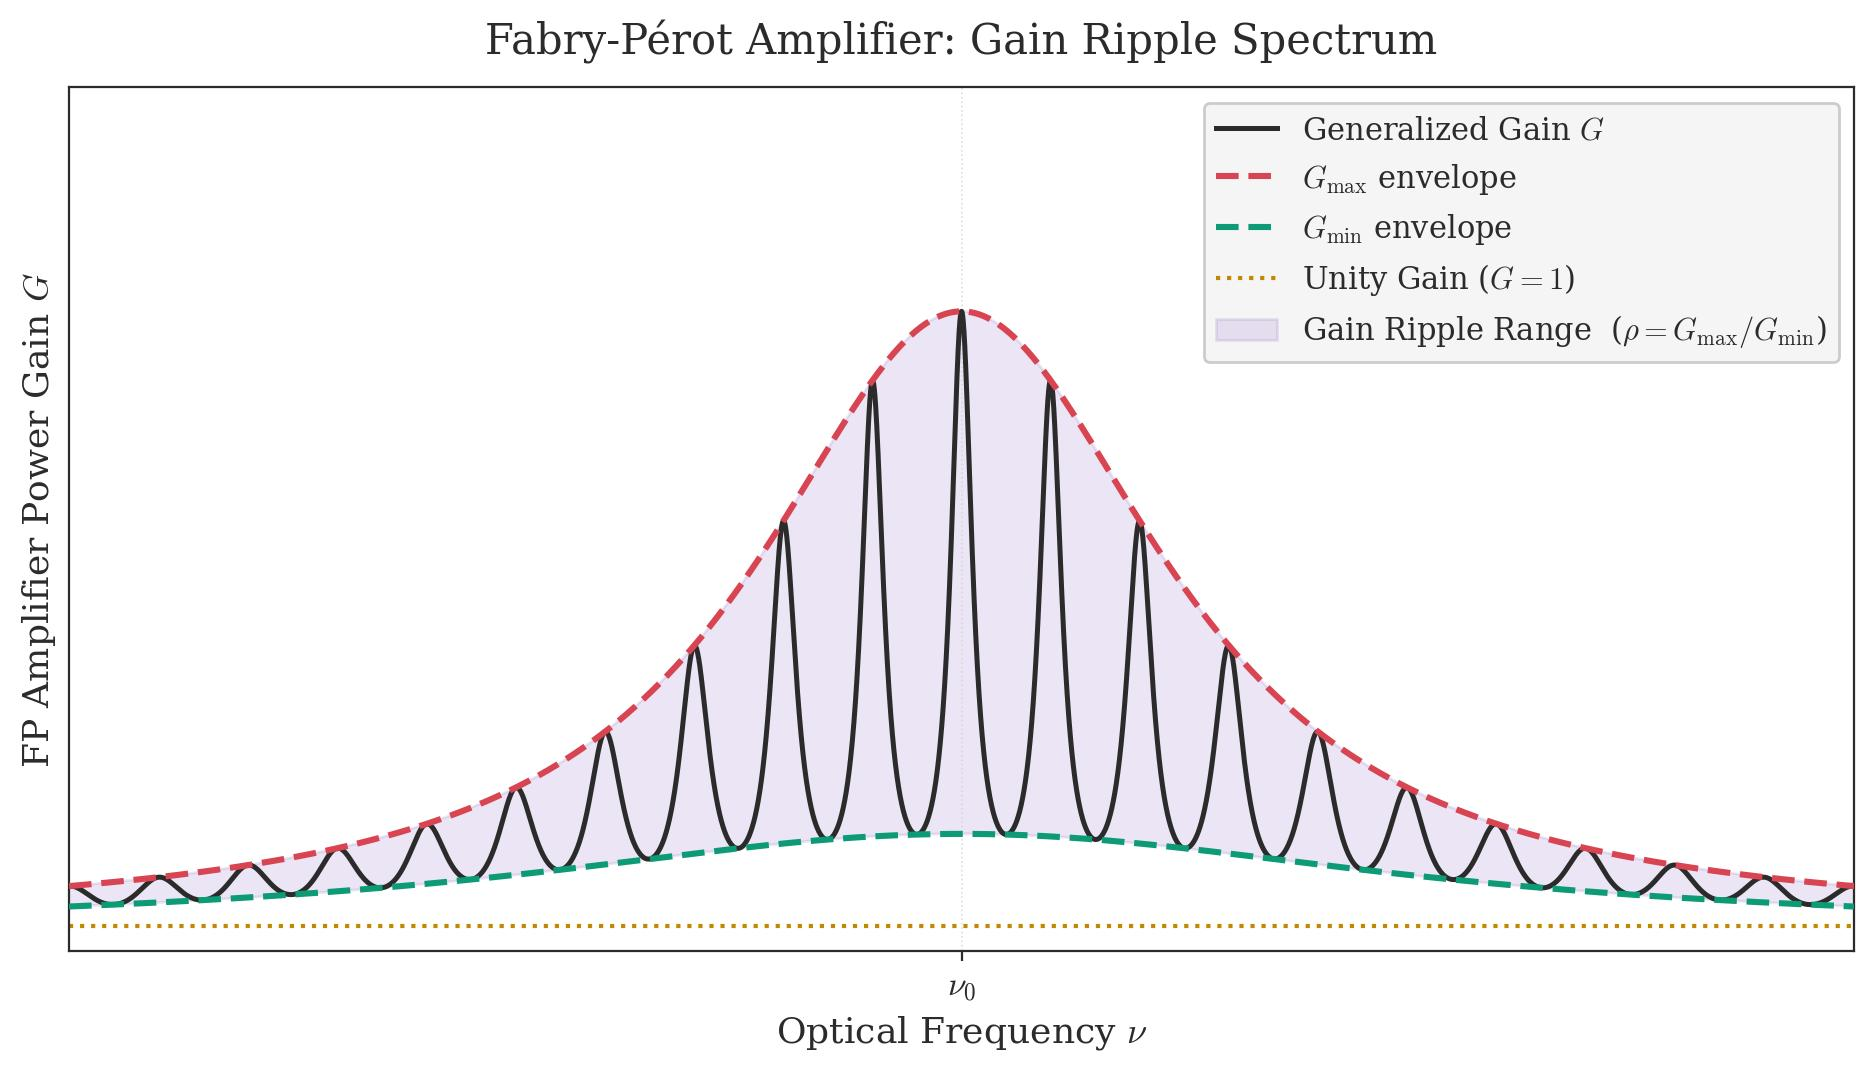
\includegraphics[width=0.6\textwidth]{Figures/Chapter 4/fp_gain_ripple_spectrum.jpg}
    \caption{Fabry-P\'{e}rot Amplifier Gain Ripple: The total power gain $G(\nu)$ oscillates between $G_\mathrm{max}$ at each cavity resonance and $G_\mathrm{min}$ at anti-resonance, with the ripple ratio growing rapidly as $G_0\sqrt{R_1 R_2}\to 1$. The near-threshold case shows dramatically sharper and taller resonance peaks --- as the round-trip gain approaches the round-trip loss, the FP amplifier converges continuously to the laser oscillator.}
\end{figure}
\subsubsection{Active bandwidth and modified finesse}

The FWHM bandwidth $\delta\nu$ of one amplified resonance peak follows from the half-power condition $G = G_{\max}/2$. The numerators cancel and the condition reduces to:
\begin{equation*}
    4\,G_0\sqrt{R_1 R_2}\,\sin^2(\beta L) = \left(1-G_0\sqrt{R_1 R_2}\right)^2
\end{equation*}

Solving for $\sin(\beta L)$, taking the inverse sine, doubling for the full FWHM, and writing $\mathrm{FSR} = c/2L$:
\begin{keyresult}
    \begin{equation}
        \delta\nu = \frac{2\,\mathrm{FSR}}{\pi}\,
        \sin^{-1}\!\left[\frac{1-G_0\sqrt{R_1 R_2}}{2\sqrt{G_0\sqrt{R_1 R_2}}}\right]
    \end{equation}
\end{keyresult}

Defining $R=\sqrt{R_1 R_2}$ as the geometric mean mirror reflectivity and applying the small-angle approximation (valid for high finesse), the ratio $\mathrm{FSR}/\delta\nu$ gives the \textbf{active finesse}:
\begin{keyresult}
    \begin{equation}
        \mathcal{F}_{\text{active}} \approx \frac{\pi\sqrt{R\,G_0}}{1-R\,G_0}
    \end{equation}
\end{keyresult}

\begin{keyinsight}[Active Finesse Reduces to Passive Finesse at Zero Gain]
    Setting $\gamma=0$ gives $G_0=e^{-\alpha_s L}$ and:
    \begin{equation*}
        \mathcal{F}_{\text{active}}\big|_{\gamma=0} = \frac{\pi\sqrt{R\,e^{-\alpha_s L}}}{1-R\,e^{-\alpha_s L}}
    \end{equation*}
    This is exactly the passive finesse expression $\pi(R_1 R_2)^{1/4}e^{-\alpha_s L/2}/(1-\sqrt{R_1 R_2}\,e^{-\alpha_s L})$ derived earlier. The active finesse is therefore a genuine generalisation --- it recovers the passive result when the gain is switched off.
\end{keyinsight}
\subsubsection{The oscillation limit}

The active finesse exceeds the passive finesse whenever $G_0 > 1$, because the gain reduces the net round-trip loss experienced by a photon. As $RG_0\to 1$ --- as we approach the oscillation threshold derived in \S1.2 --- the active finesse diverges and the resonance peaks become arbitrarily narrow. At that crossing, the gain-to-infinity condition is met, and what was a sub-threshold amplifier becomes, precisely, the laser oscillator.

The laser physics is now complete at the amplitude and rate-equation level: we know the threshold, the surviving modes, and the steady-state output power. One final assumption deserves scrutiny: we have treated the gain medium as a pure amplitude element, leaving the lasing frequencies unchanged from their cold-cavity values. That is not quite correct. The gain medium also introduces a phase shift, and that phase shift pulls the real oscillation frequencies away from the cold-cavity comb.

% ----------------------------------------------------------
%  Section 4: The Hot Resonator
% ----------------------------------------------------------
\section{The Hot Resonator: Frequency Pulling and Chirping}

So far we have assumed that the resonance frequencies are the cold-cavity values $\nu_q = qc/(2L)$, determined purely by geometry. But we forgot something important: the gain medium inside the cavity also introduces a \emph{phase shift} --- not just amplitude gain. This is a direct consequence of the Kramers-Kronig relations, which link the real and imaginary parts of the complex susceptibility. We cannot have gain (imaginary part) without also having an accompanying change in the refractive index (real part), and that index change modifies the round-trip phase.

\subsection{Kramers-Kronig and Phase Shift from the Gain Medium}

The complex susceptibility of the gain medium has a real part $\chi'$ (dispersion, causes a phase shift) and an imaginary part $\chi''$ (gain or absorption). Close to resonance, these satisfy:
\begin{equation*}
    \chi'' \propto \gamma \qquad\text{(related to gain)}
\end{equation*}
\begin{equation*}
    \chi' = \frac{2(\nu - \nu_0)}{\Delta\nu}\,\chi'' \qquad\text{(Kramers-Kronig near resonance)}
\end{equation*}

The susceptibility $\chi'$ modifies the effective propagation constant. The gain medium adds an extra phase increment $\Delta\beta$ per unit length to the cold-cavity phase constant:
\begin{keyresult}
    \begin{equation}
        \Delta\beta = \left(\frac{\nu - \nu_0}{\Delta\nu}\right)\gamma
    \end{equation}
\end{keyresult}

$\Delta\beta = 0$ at line centre $\nu = \nu_0$ --- the gain introduces no extra phase at the atomic resonance itself. Off-resonance, $\Delta\beta$ is proportional to both the detuning from line centre and the gain coefficient.

\subsection{Modified Phase Condition --- The Hot Resonator}

The total propagation constant inside the cavity is now $\beta + \Delta\beta$. The modified round-trip phase condition becomes:
\begin{equation*}
    2(\beta + \Delta\beta)L = 2q\pi
\end{equation*}

Substituting $\beta = 2\pi\nu/c$ and $\Delta\beta$:
\begin{equation*}
    \frac{2\nu L}{c} + \frac{(\nu - \nu_0)}{\pi\Delta\nu}\,\gamma L = q
\end{equation*}

The oscillation frequency $\nu'_q$ (the ``hot-resonator'' mode frequency) is the solution of this equation, and in general it differs from the cold-resonator mode $\nu_q = qc/(2L)$.

\subsection{Frequency Pulling}

To understand how $\nu'_q$ differs from $\nu_q$, consider the dispersive profile of $\Delta\beta$: it is negative for $\nu < \nu_0$ (below resonance) and positive for $\nu > \nu_0$ (above resonance). For modes below $\nu_0$, the extra phase \emph{decreases} the effective propagation constant, which makes the cavity look optically shorter --- the mode frequency shifts \emph{up} toward $\nu_0$. For modes above $\nu_0$, the reverse occurs and the mode shifts \emph{down} toward $\nu_0$.

The net effect is that all hot-resonator modes $\nu'_q$ are \textbf{pulled toward the atomic resonance $\nu_0$} relative to the cold-resonator modes $\nu_q$. This phenomenon is called \textbf{frequency pulling}. We can derive the exact pulled frequency explicitly. Recall from the modified phase condition:
\begin{equation*}
    \frac{2\nu'_q L}{c} + \frac{(\nu'_q - \nu_0)}{\pi\Delta\nu}\,\gamma L = q
\end{equation*}
The cold-resonator mode satisfies $2\nu_q L/c = q$ exactly, so we substitute $q = 2\nu_q L/c$ and collect terms in $\nu'_q$:
\begin{equation*}
    \nu'_q\!\left[\frac{2L}{c} + \frac{\gamma L}{\pi\Delta\nu}\right] = \frac{2\nu_q L}{c} + \frac{\nu_0\,\gamma L}{\pi\Delta\nu}
\end{equation*}
Dividing through by $L$ and defining the dimensionless pulling parameter $P = c\gamma/(2\pi\Delta\nu)$:
\begin{equation*}
    \nu'_q\!\left[\frac{2}{c} + \frac{\gamma}{\pi\Delta\nu}\right] = \frac{2\nu_q}{c} + \frac{\nu_0\,\gamma}{\pi\Delta\nu}
    \quad\implies\quad
    \nu'_q\,(1 + P) = \nu_q + P\,\nu_0
\end{equation*}
Solving for the hot-resonator mode frequency:
\begin{keyresult}
    \begin{equation}
        \nu'_q = \frac{\nu_q + P\,\nu_0}{1 + P}, \qquad P = \frac{c\gamma}{2\pi\,\Delta\nu}
    \end{equation}
\end{keyresult}
where:
\begin{itemize}
    \item $\nu'_q$: the actual lasing frequency of the $q$-th mode (hot-resonator value).
    \item $\nu_q = qc/(2L)$: the geometric cold-resonator mode frequency.
    \item $P = c\gamma/(2\pi\Delta\nu)$: a dimensionless ratio of gain to atomic linewidth. It quantifies how strongly the gain medium perturbs the cavity modes.
\end{itemize}

The pulling amount --- how far $\nu'_q$ shifts from $\nu_q$ --- is:
\begin{equation*}
    \nu'_q - \nu_q = \frac{P\,(\nu_0 - \nu_q)}{1 + P}
    \xrightarrow{\;P\ll 1\;}
    P\,(\nu_0 - \nu_q) = \frac{c\gamma}{2\pi\Delta\nu}\,(\nu_0 - \nu_q)
\end{equation*}

The pulling is proportional to both the gain coefficient $\gamma$ and the cold-cavity detuning $(\nu_0 - \nu_q)$. Modes already close to line centre ($\nu_q \approx \nu_0$) are barely pulled; modes at the edges of the gain profile feel the strongest pull. In the limit $P \to \infty$ (gain much larger than the linewidth), the formula gives $\nu'_q \to \nu_0$ for every mode --- the entire mode comb would collapse to line centre, a physically unreachable limit that nevertheless confirms the direction of the effect.

\begin{figure}[H]
    \centering
    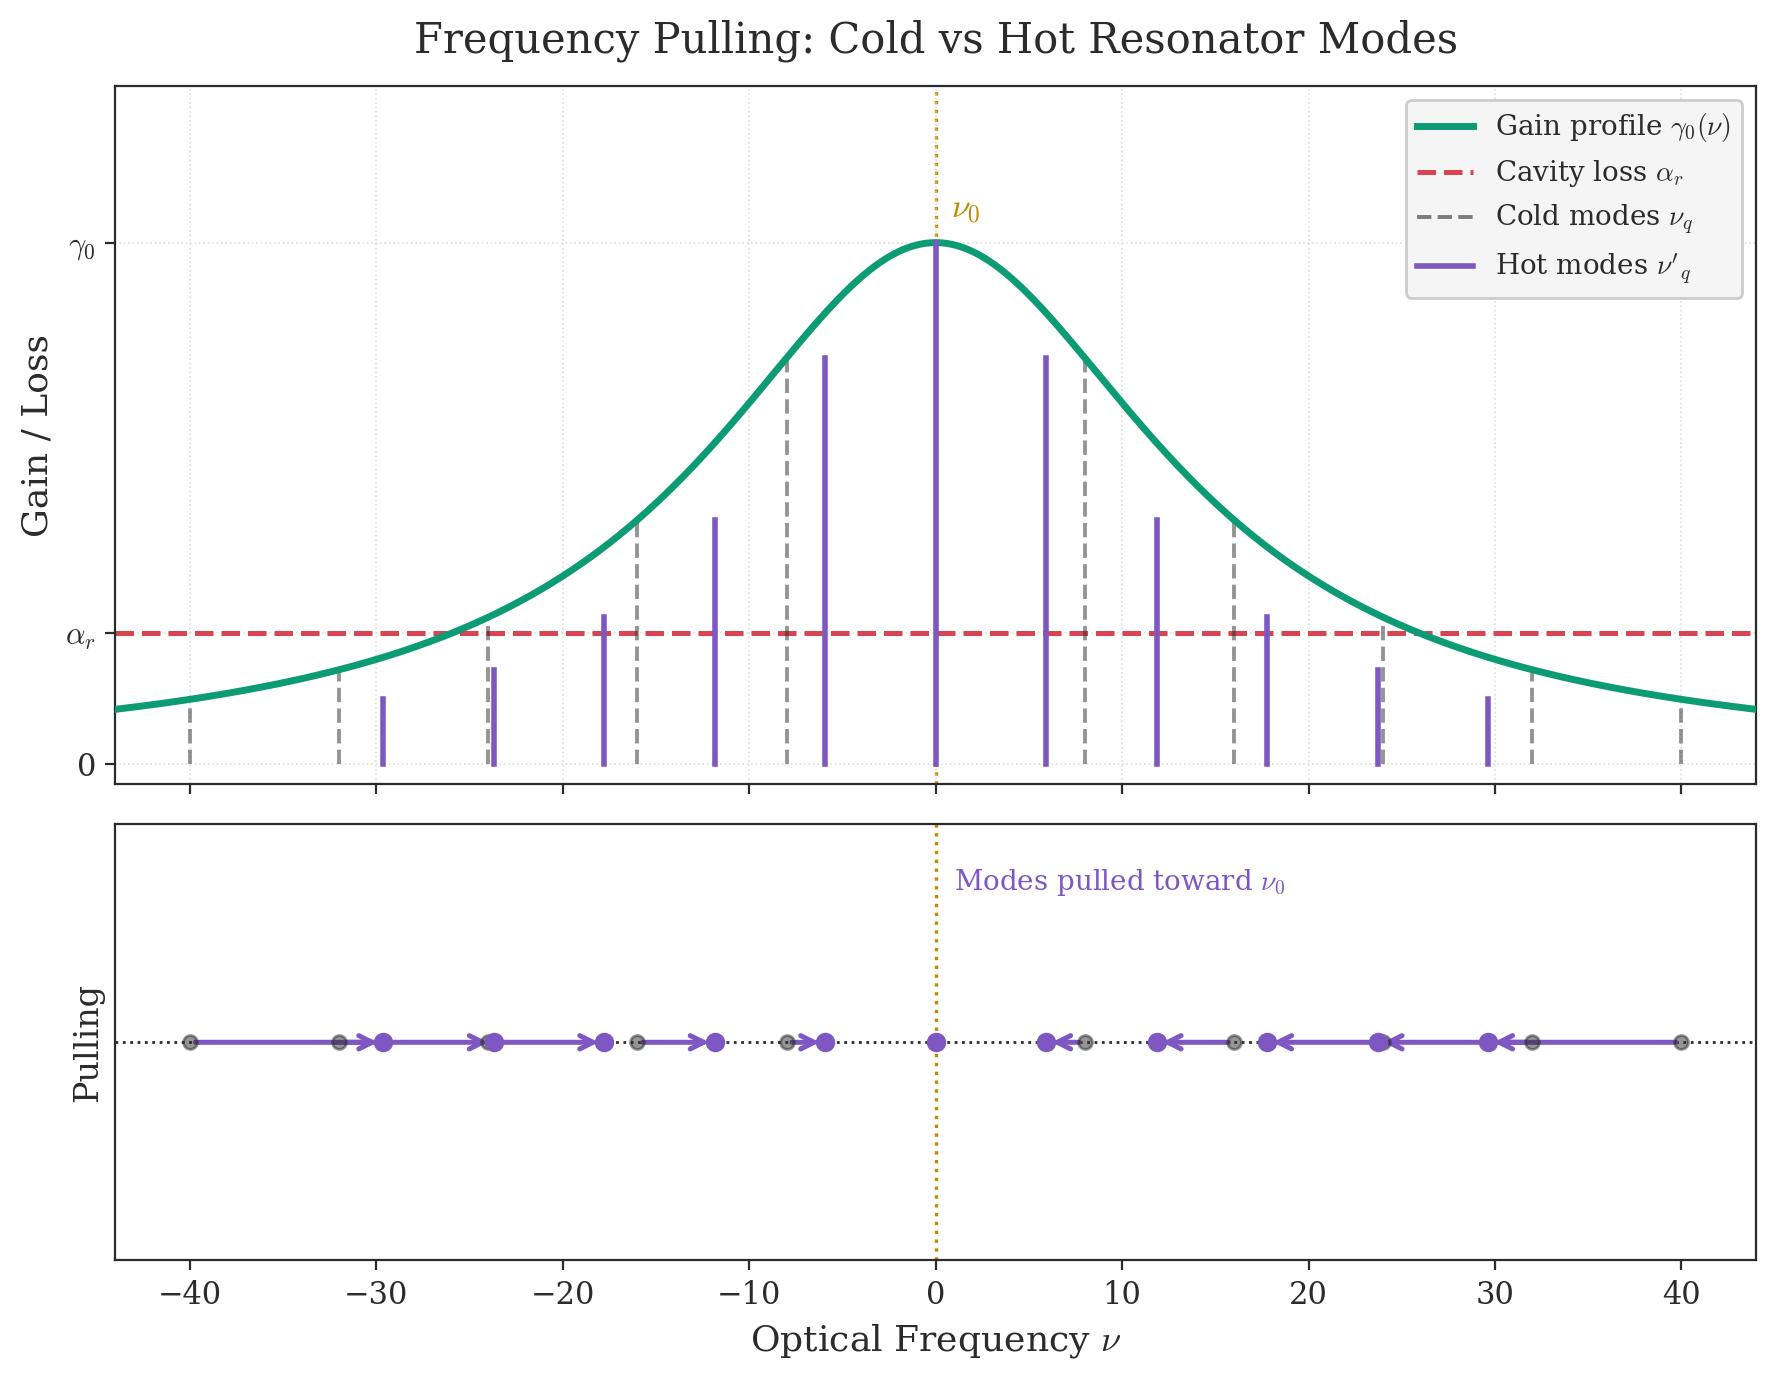
\includegraphics[width=0.7\textwidth]{Figures/Chapter 4/frequency_pulling_diagram.jpg}
    \caption{Frequency Pulling --- Cold vs.~Hot Resonator: The cold-resonator modes (dashed lines) are evenly spaced at the geometric frequencies $\nu_q = qc/(2L)$. The gain medium introduces a dispersive phase shift $\Delta\beta$ that is antisymmetric about $\nu_0$, pulling each mode toward the atomic resonance. The hot-resonator modes (solid lines) sit at $\nu'_q = (\nu_q + P\nu_0)/(1+P)$, all displaced inward relative to the gain profile centre.}
\end{figure}

\begin{keyinsight}[Cold vs Hot Resonator Frequencies]
    The cold-resonator modes at $\nu_q = qc/(2L)$ are determined purely by cavity geometry. The hot-resonator modes $\nu'_q$ --- the actual oscillation frequencies of the running laser --- are pulled slightly toward the atomic resonance $\nu_0$. The amount of pulling depends on how far $\nu_q$ is from $\nu_0$ and on the magnitude of the gain. This is why a real laser oscillates at frequencies that are close to, but measurably offset from, the purely geometric cold-cavity frequencies. The dispersive Kramers-Kronig phase shift from the gain medium inevitably acts as a force dragging the oscillation toward line centre.
\end{keyinsight}

\subsection{Direct Laser Modulation and Frequency Chirping}

The most practically impactful consequence of frequency pulling arises when the laser is used as a directly modulated transmitter. In direct laser modulation, digital data is encoded by varying the injection current (or pump rate) to swing the output power between a high level (logical~1) and a low level (logical~0). This approach is operationally elegant: no external optical component is required beyond the laser itself.

Frequency pulling, however, immediately identifies a fundamental side-effect. The injection current directly controls the population inversion $N_0$, which sets the gain coefficient $\gamma$. As we have just derived, any change in $\gamma$ simultaneously forces a change in the real part of the susceptibility through the Kramers-Kronig relation, and therefore a change in the intracavity refractive index $n$. A change in $n$ modifies the optical path length inside the cavity, which in turn shifts the resonant mode frequencies. The operating frequency of the laser therefore does not stay fixed during modulation --- it shifts in synchrony with the amplitude.

This unwanted coupling between amplitude modulation and frequency modulation is called \textbf{frequency chirping}. During the rising edge of a transmitted pulse --- when the pump current increases, the gain rises, and the refractive index shifts --- the lasing frequency swings in one direction. During the falling edge, it swings back. The instantaneous optical frequency therefore oscillates up and down in synchrony with the amplitude waveform, broadening the emitted spectrum far beyond what the pure modulation bandwidth alone would predict.

\begin{keyinsight}[Why Chirping Limits Long-Haul Communication]
    A chirped optical pulse carries a range of frequencies that travel at slightly different speeds through a dispersive fibre. This differential propagation speed causes the pulse to spread in time as it travels, eventually causing adjacent pulses to overlap and become indistinguishable at the receiver. The faster the modulation and the more dispersive the fibre, the shorter the usable transmission distance. For this reason, all high-speed, long-haul optical communication systems avoid direct laser modulation entirely, using instead an external modulator (typically a Mach-Zehnder interferometer) that varies the light's amplitude without touching the laser's injection current, leaving the gain and refractive index undisturbed and keeping the output frequency stable.
\end{keyinsight}

\begin{figure}[H]
    \centering
    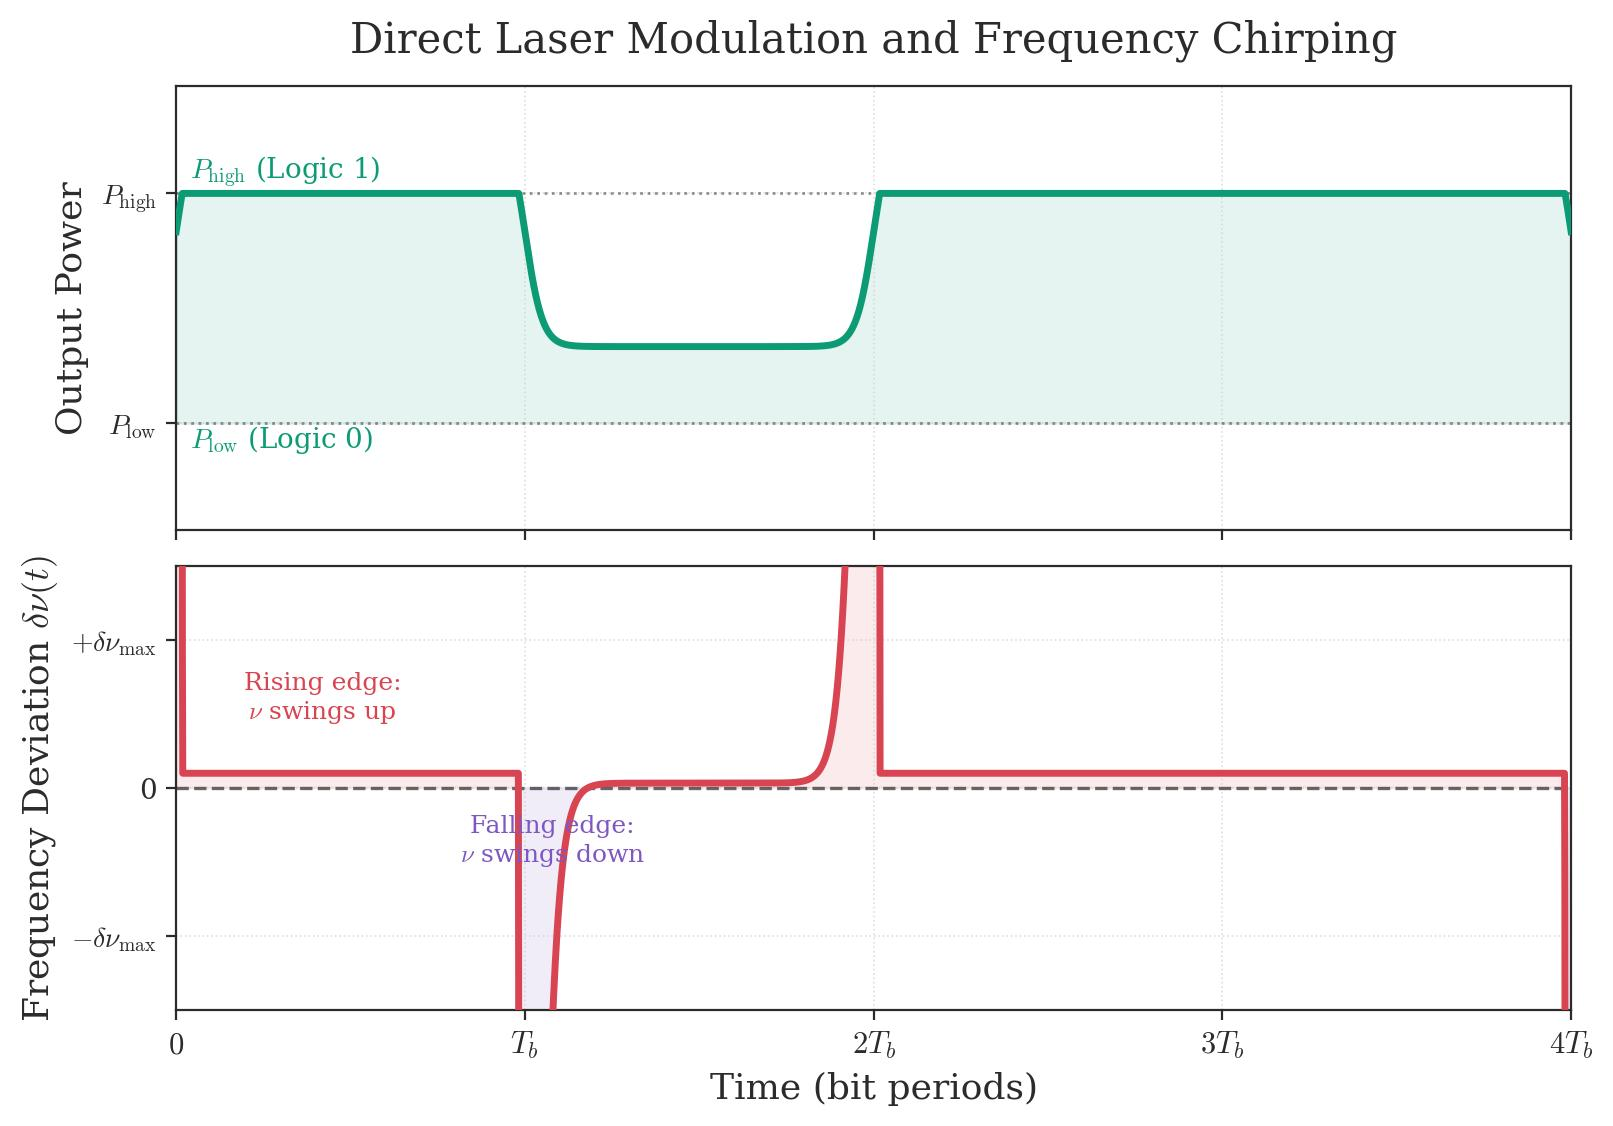
\includegraphics[width=0.7\textwidth]{Figures/Chapter 4/frequency_chirping.jpg}
    \caption{Direct Laser Modulation and Frequency Chirping: (Top) The optical output power follows the modulation pattern, switching between logical high and low levels. (Bottom) The instantaneous lasing frequency is not constant --- it swings up during the rising edge (gain increasing $\to$ refractive index shifting) and down during the falling edge, tracing the amplitude modulation pattern. This unwanted frequency deviation is frequency chirping; it broadens the signal spectrum and limits usable transmission distance over dispersive fibres.}
\end{figure}

% =============================================================
\section*{From General Theory to Semiconductor Realities}
% =============================================================

Throughout this chapter, we have built a rigorous macroscopic model of the laser oscillator. By introducing optical feedback via the Fabry-P\'{e}rot cavity, we successfully constructed a self-sustaining device that requires no external seed signal. We quantified the oscillation threshold, analysed the spatial modes determined by cavity mechanics, explored the mode competition driven by homogeneous versus inhomogeneous broadening, calculated the steady-state output power derived from gain saturation, and finally uncovered the subtle coupling between gain and phase that causes frequency pulling and chirping in real operating lasers.

However, a fundamental abstraction remains at the core of our oscillator model: \textbf{we have treated the gain medium as a generic collection of isolated atoms}. In reality, the most transformative and widely deployed lasers in the modern world --- from the fibre-optic backbone of the internet to the barcode scanner --- do not use isolated atoms floating in a gas. They use tightly packed crystal lattices where billions of atoms interact continuously. A generic atomic model cannot systematically explain how to inject carriers into these bands or how a simple electrical current produces optical gain.

\begin{keyinsight}[The Missing Physics: Solid-State Semiconductors]
    To transform our theoretical oscillator into the immensely practical, electrically driven devices that dominate modern optoelectronics, we must introduce \textbf{semiconductor physics}.

    If we replace the generic atomic gas with a semiconductor PN junction, the discrete energy levels blur into continuous energy bands. Instead of pumping isolated atoms with external light, we can directly inject massive populations of electrons and holes across the junction using a simple forward bias. By physically trapping these massive carrier populations in a confined region, we can achieve the necessary population inversion entirely through electrical means.
\end{keyinsight}

This conceptual leap from a generic atomic cavity to a solid-state, electrically driven diode is the ultimate transition into applied optoelectronics. The cavity mechanics we have mastered here --- threshold conditions, mode spacing, and photon lifetimes --- will now serve as the structural framework housing this new semiconductor gain medium. The next chapter will review exactly how this band-structure physics successfully powers the LED and the \textbf{semiconductor laser diode}.


